\documentclass{article}

\usepackage{graphicx}
\usepackage{amsmath}
\usepackage{fancyhdr}
\usepackage{float}
\usepackage{titlesec}
\usepackage[sorting=none]{biblatex}
\usepackage[margin=1in]{geometry}
\usepackage[font={small,it}]{caption}
\usepackage{placeins}
\usepackage{xepersian}

%\DeclareMathOperator*{\btie}{\bowtie}
\addbibresource{bibliography.bib}
\settextfont[Scale=1.2]{B-NAZANIN.TTF}
\setlatintextfont[Scale=1]{Times New Roman}
\renewcommand{\baselinestretch}{1.5}
\pagestyle{fancy}
\fancyhf{}
\rhead{تکلیف چهارم آزمایشگاه شبکه ‌های کامپیوتری}
\lhead{\thepage}
\rfoot{علیرضا ابره فروش}
\lfoot{9816603}
\renewcommand{\headrulewidth}{1pt}
\renewcommand{\footrulewidth}{1pt}

\begin{document}
\begin{titlepage}
\begin{center}

\includegraphics[width=0.4\textwidth]{figures/IUT Logo.png}\\
        
\LARGE
\textbf{دانشگاه صنعتی اصفهان}\\
\textbf{دانشکده مهندسی برق و کامپیوتر}\\
        
\vfill
        
\huge
\textbf{عنوان: تکلیف چهارم درس ریزپردازنده}\\
        
\vfill
        
\LARGE
\textbf{نام و نام خانوادگی: علیرضا ابره فروش}\\
\textbf{شماره دانشجویی: 9816603}\\
\textbf{نیم\,سال تحصیلی: پاییز 1400}\\
\textbf{مدرّس: دکتر عارف کریمی افشار}\\
\end{center}
\end{titlepage}


%\tableofcontents
\newpage



\section{}
\subsection{}
\begin{figure}[H]
    \centering
    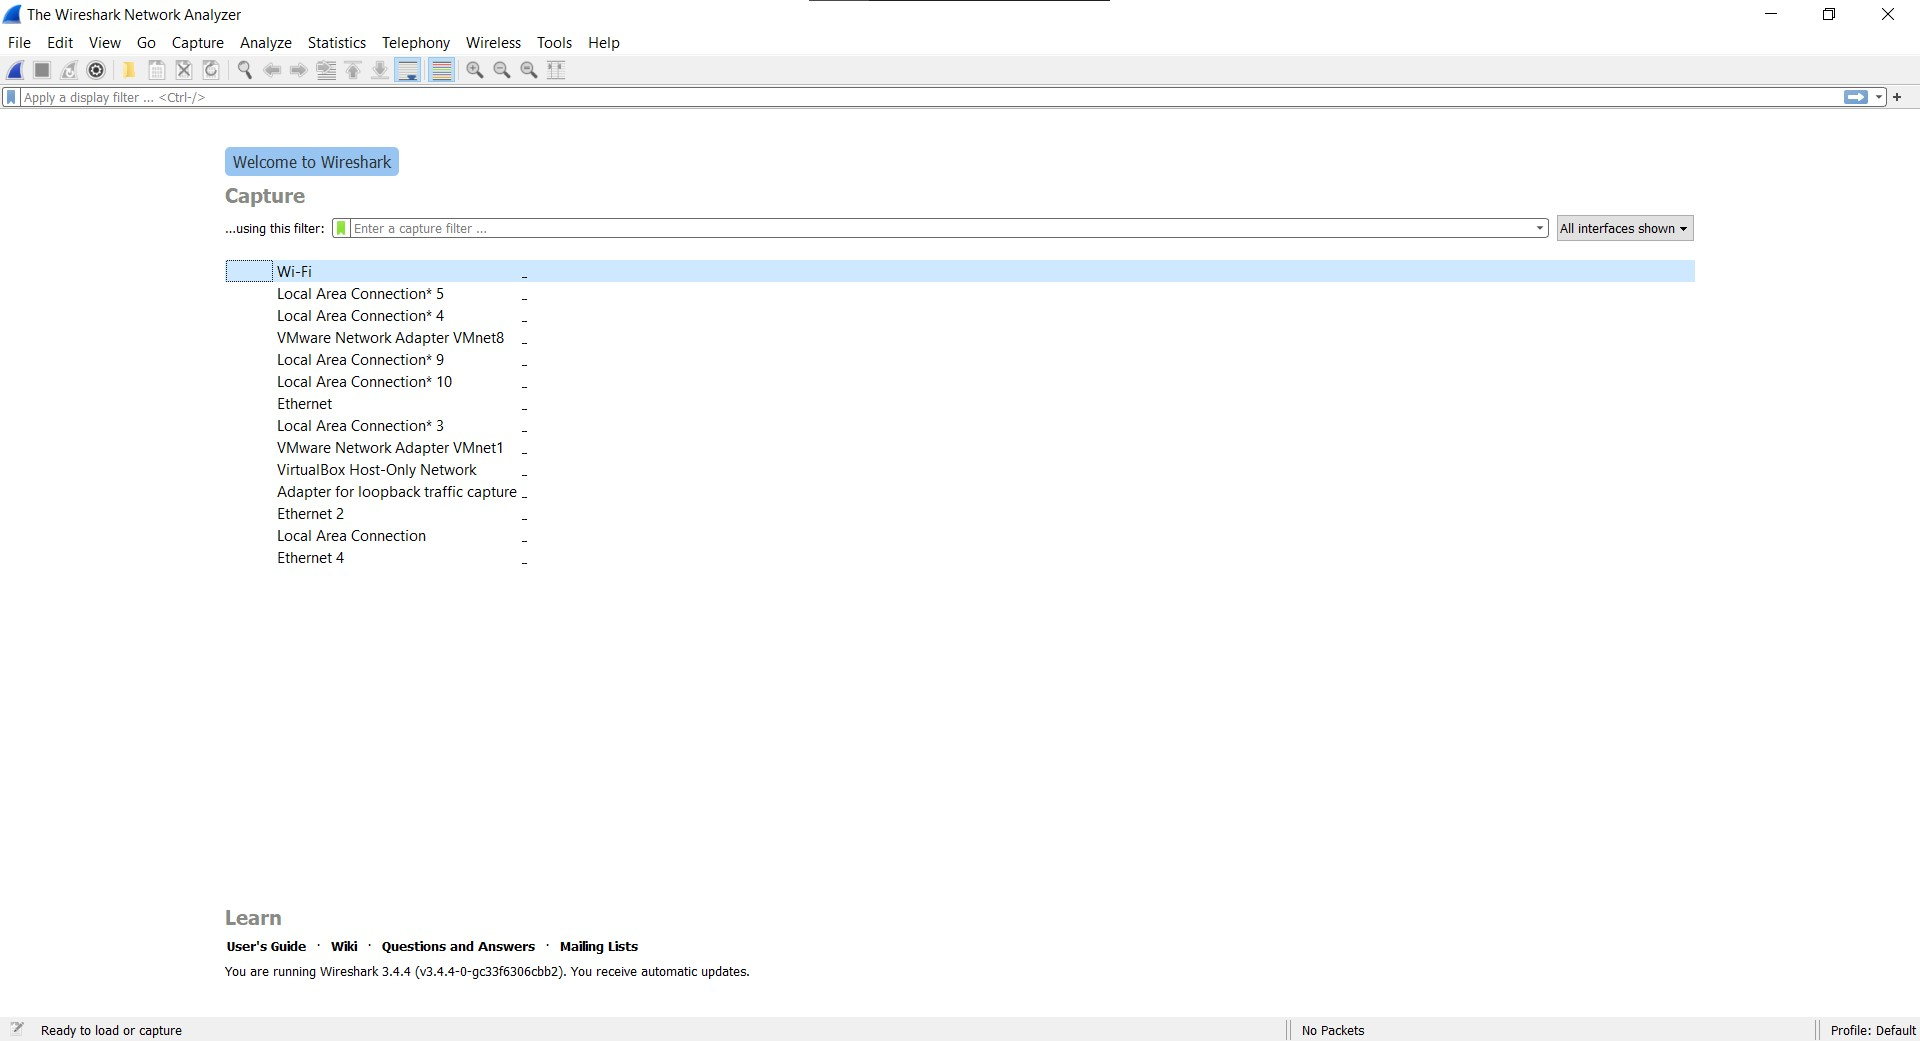
\includegraphics[width=1.0\textwidth]{figures/1.jpg}
    \caption{}
    \label{fig:fig1}
\end{figure}

\begin{figure}[H]
    \centering
    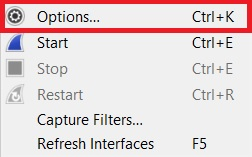
\includegraphics[width=0.5\textwidth]{figures/2.jpg}
    \caption{}
    \label{fig:fig1}
\end{figure}

\begin{figure}[H]
    \centering
    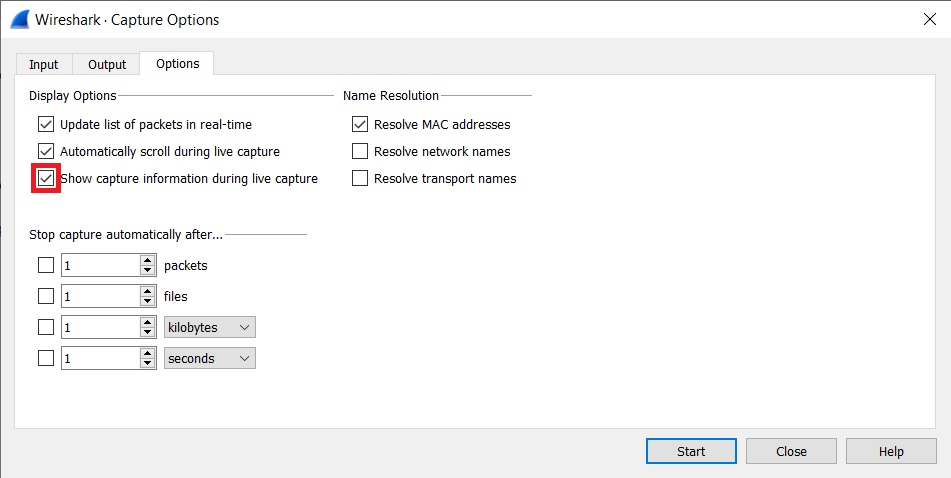
\includegraphics[width=1.0\textwidth]{figures/3.jpg}
    \caption{}
    \label{fig:fig1}
\end{figure}

\begin{figure}[H]
    \centering
    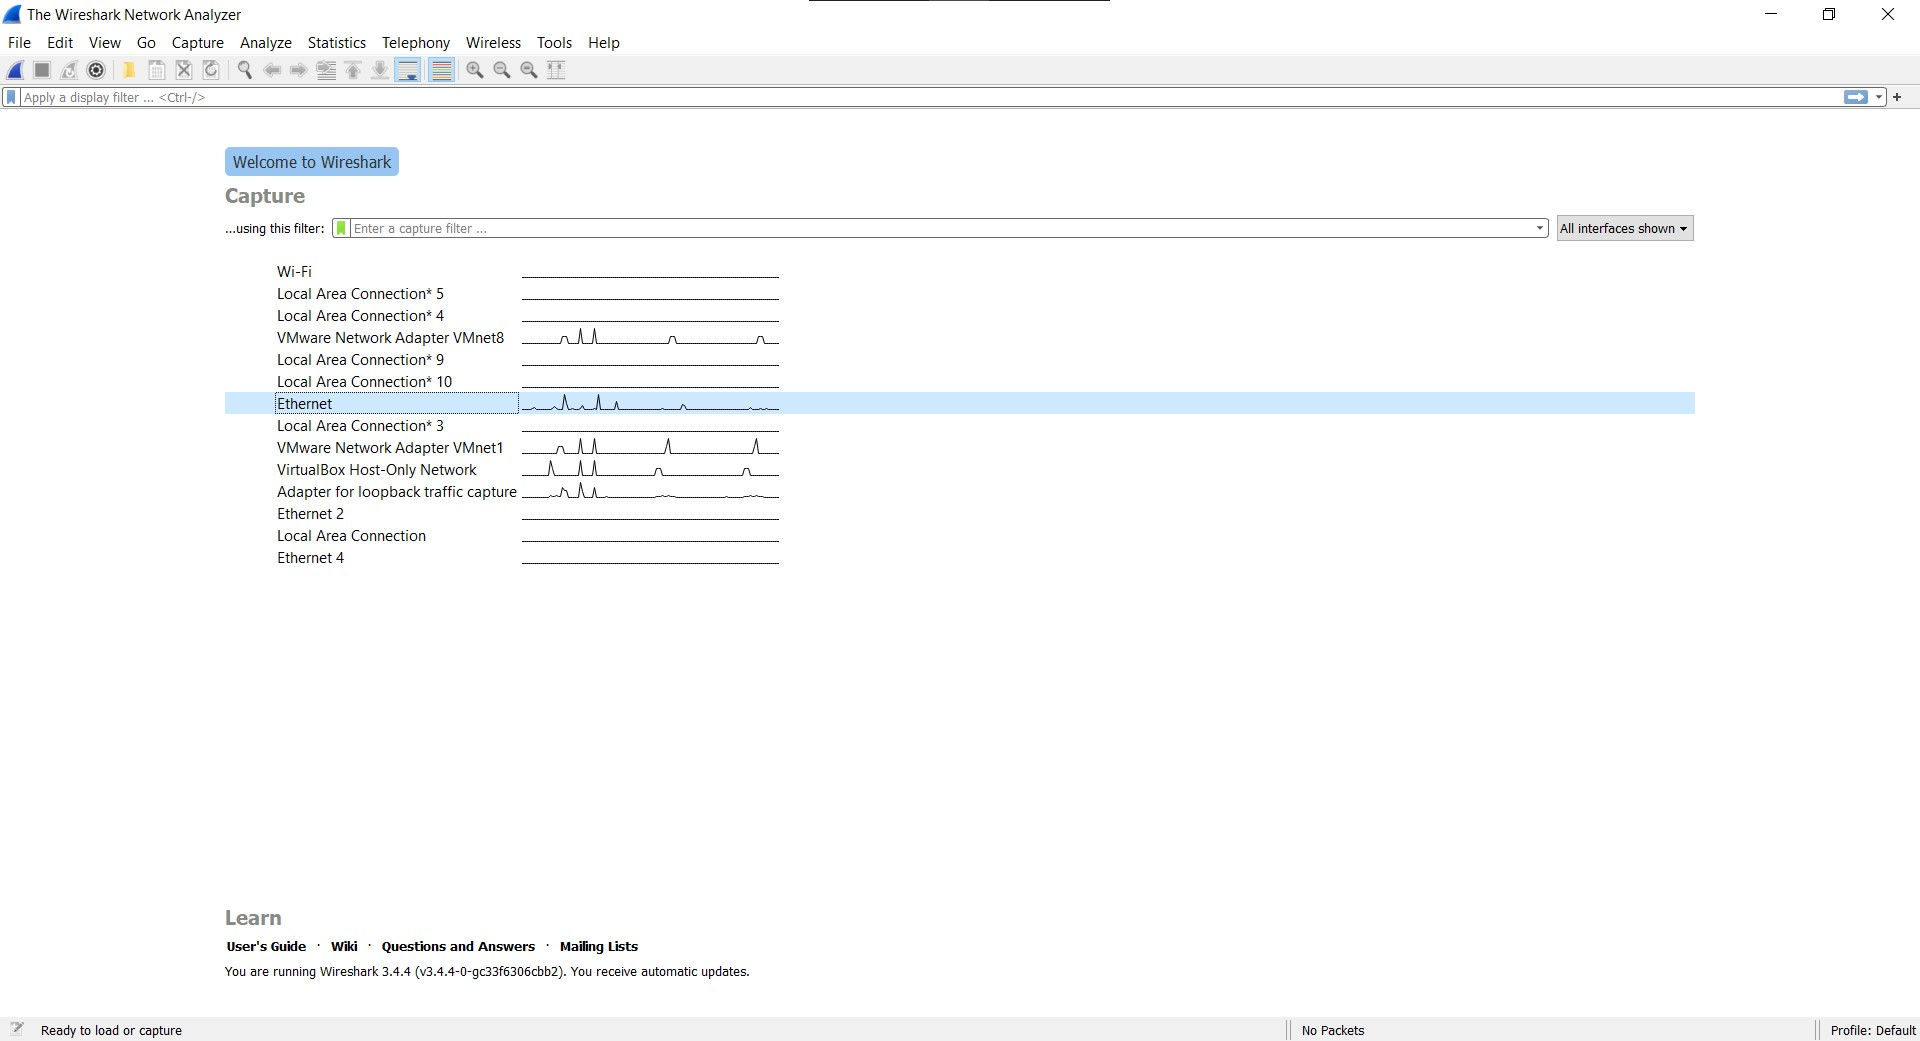
\includegraphics[width=1.0\textwidth]{figures/4.jpg}
    \caption{}
    \label{fig:fig1}
\end{figure}

\begin{figure}[H]
    \centering
    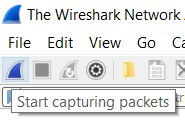
\includegraphics[width=0.5\textwidth]{figures/5.jpg}
    \caption{}
    \label{fig:fig1}
\end{figure}

\begin{figure}[H]
    \centering
    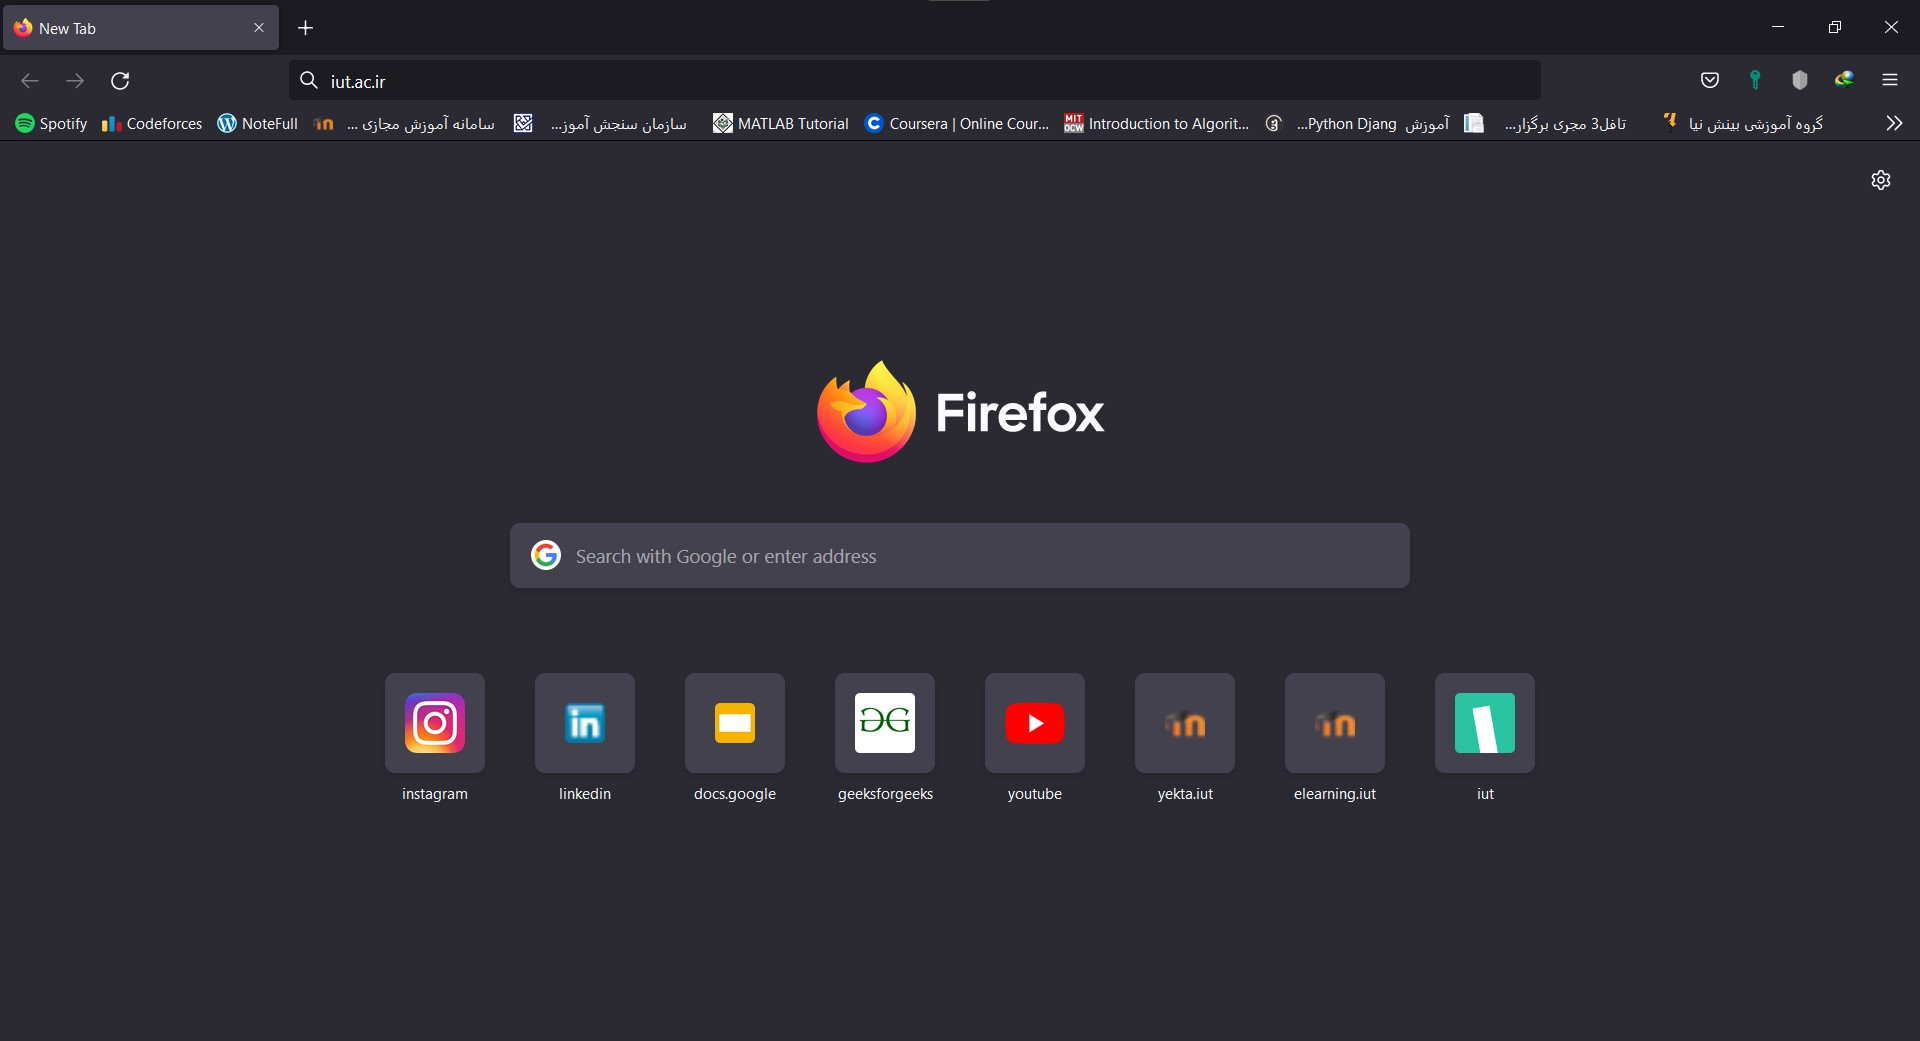
\includegraphics[width=1.0\textwidth]{figures/6.jpg}
    \caption{}
    \label{fig:fig1}
\end{figure}

\begin{figure}[H]
    \centering
    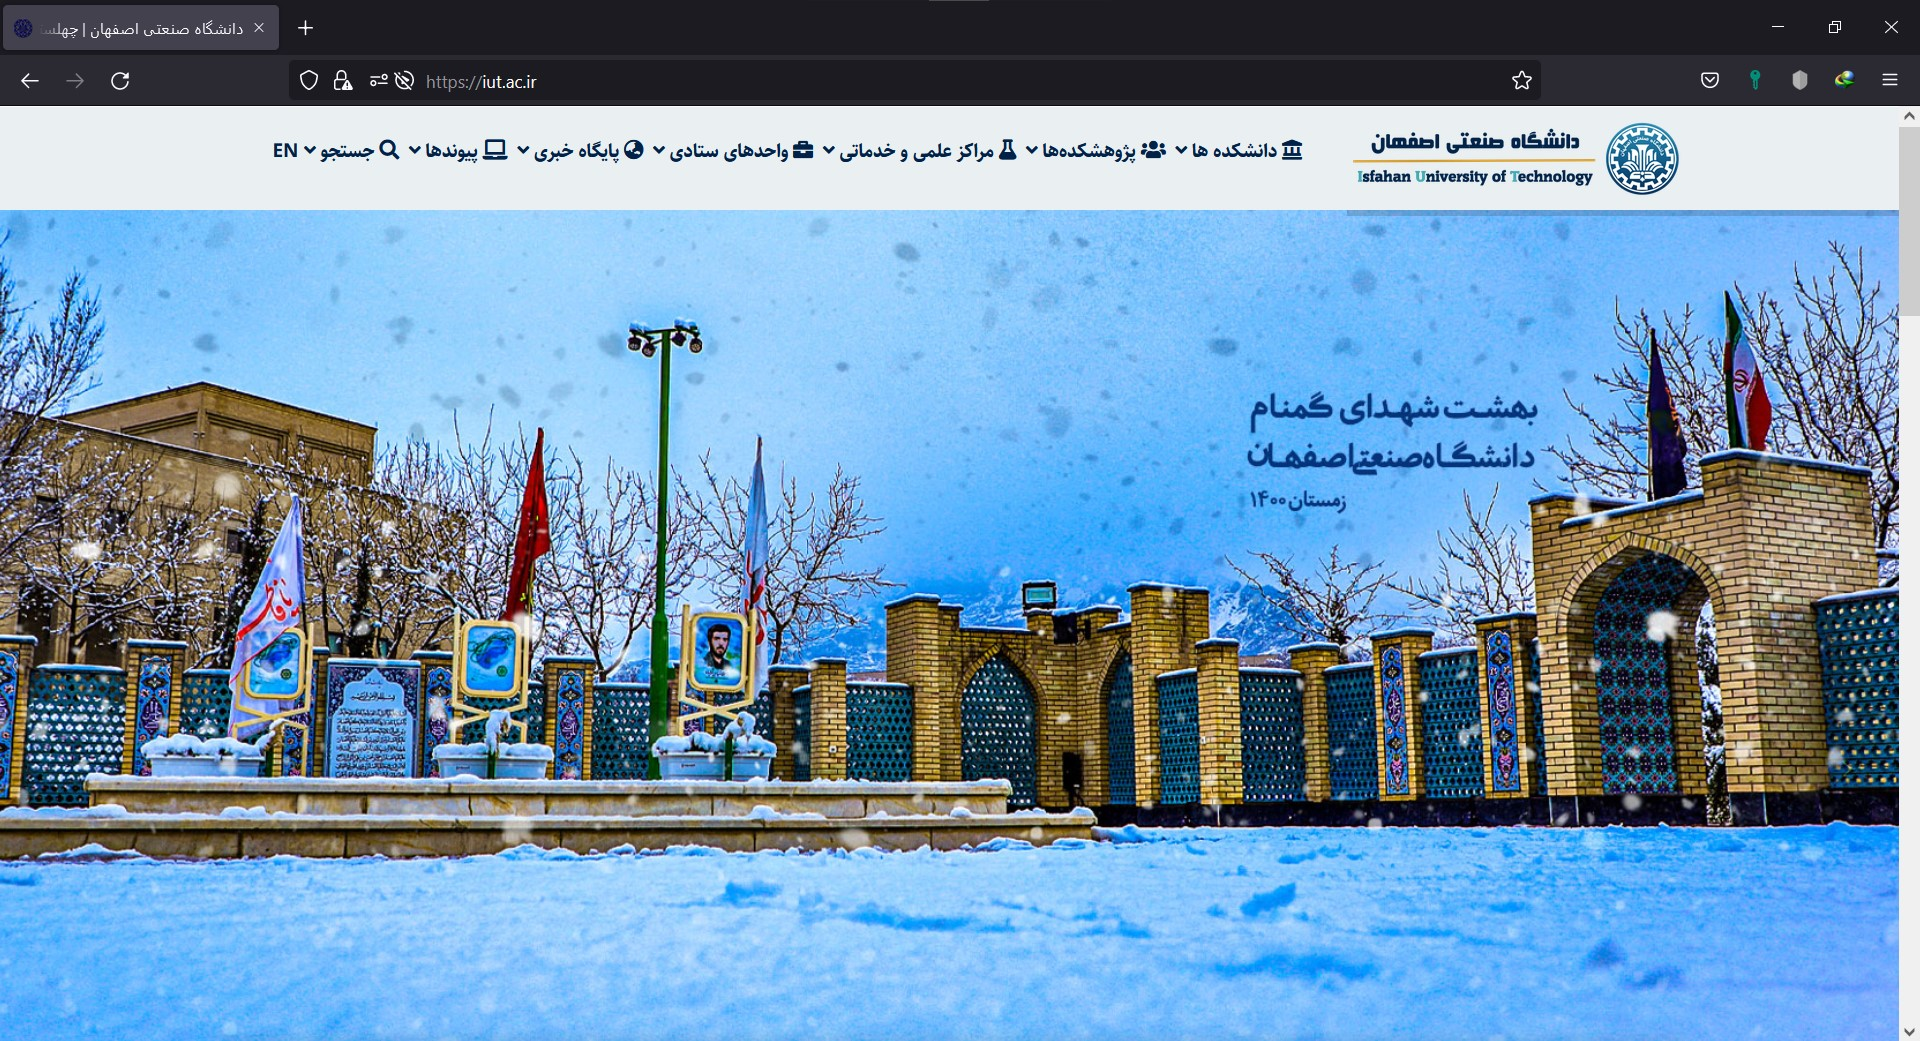
\includegraphics[width=1.0\textwidth]{figures/7.jpg}
    \caption{}
    \label{fig:fig1}
\end{figure}

\begin{figure}[H]
    \centering
    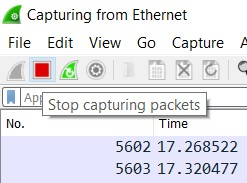
\includegraphics[width=0.5\textwidth]{figures/8.jpg}
    \caption{}
    \label{fig:fig1}
\end{figure}

\begin{figure}[H]
    \centering
    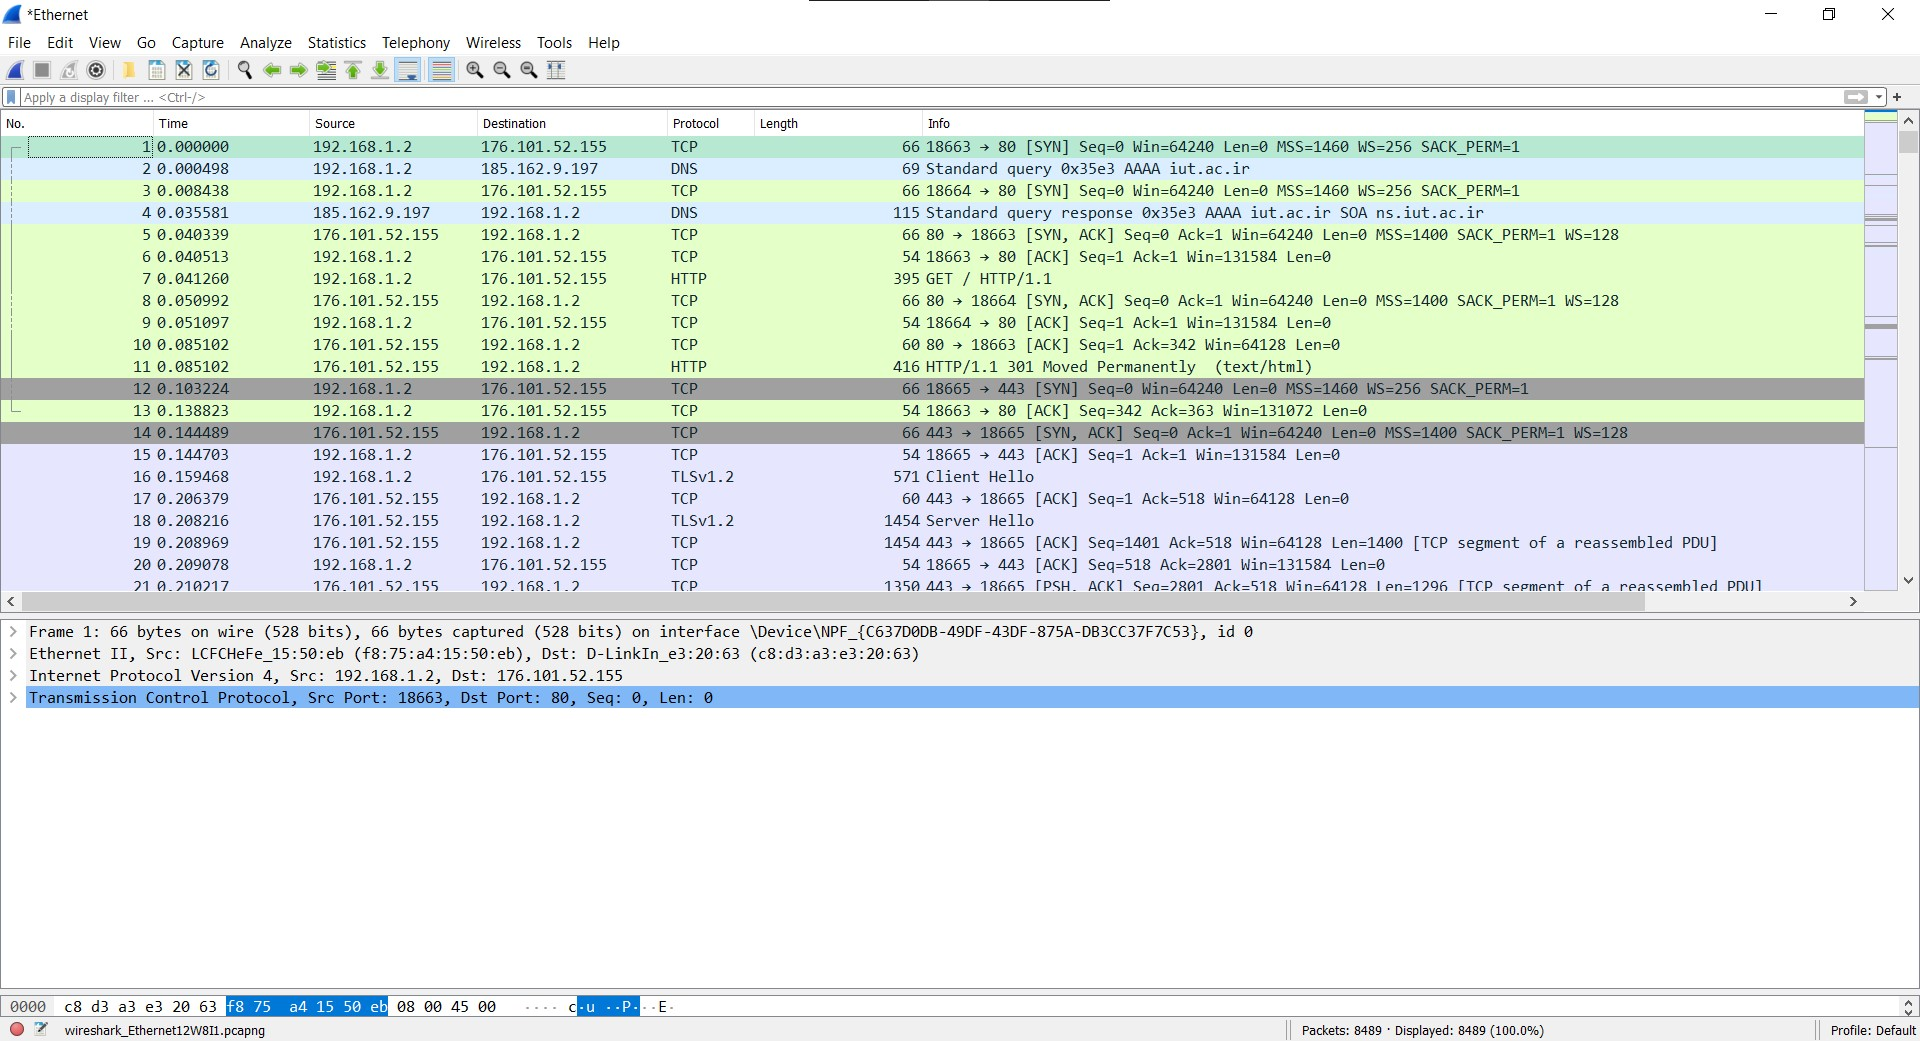
\includegraphics[width=1.0\textwidth]{figures/9.jpg}
    \caption{}
    \label{fig:fig1}
\end{figure}
پروتکل‌های زیر دیده می‌شوند:
\begin{itemize}
	\item [$\bullet$] \lr{TCP}
	\item [$\bullet$] \lr{DNS}
	\item [$\bullet$] \lr{HTTP}
	\item [$\bullet$] \lr{TLSv1.2}
	\item [$\bullet$] \lr{ICMP}
\end{itemize}


\subsection{}
\begin{figure}[H]
    \centering
    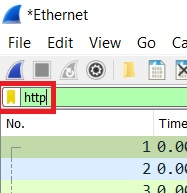
\includegraphics[width=0.5\textwidth]{figures/11.jpg}
    \caption{}
    \label{fig:fig1}
\end{figure}
\begin{figure}[H]
    \centering
    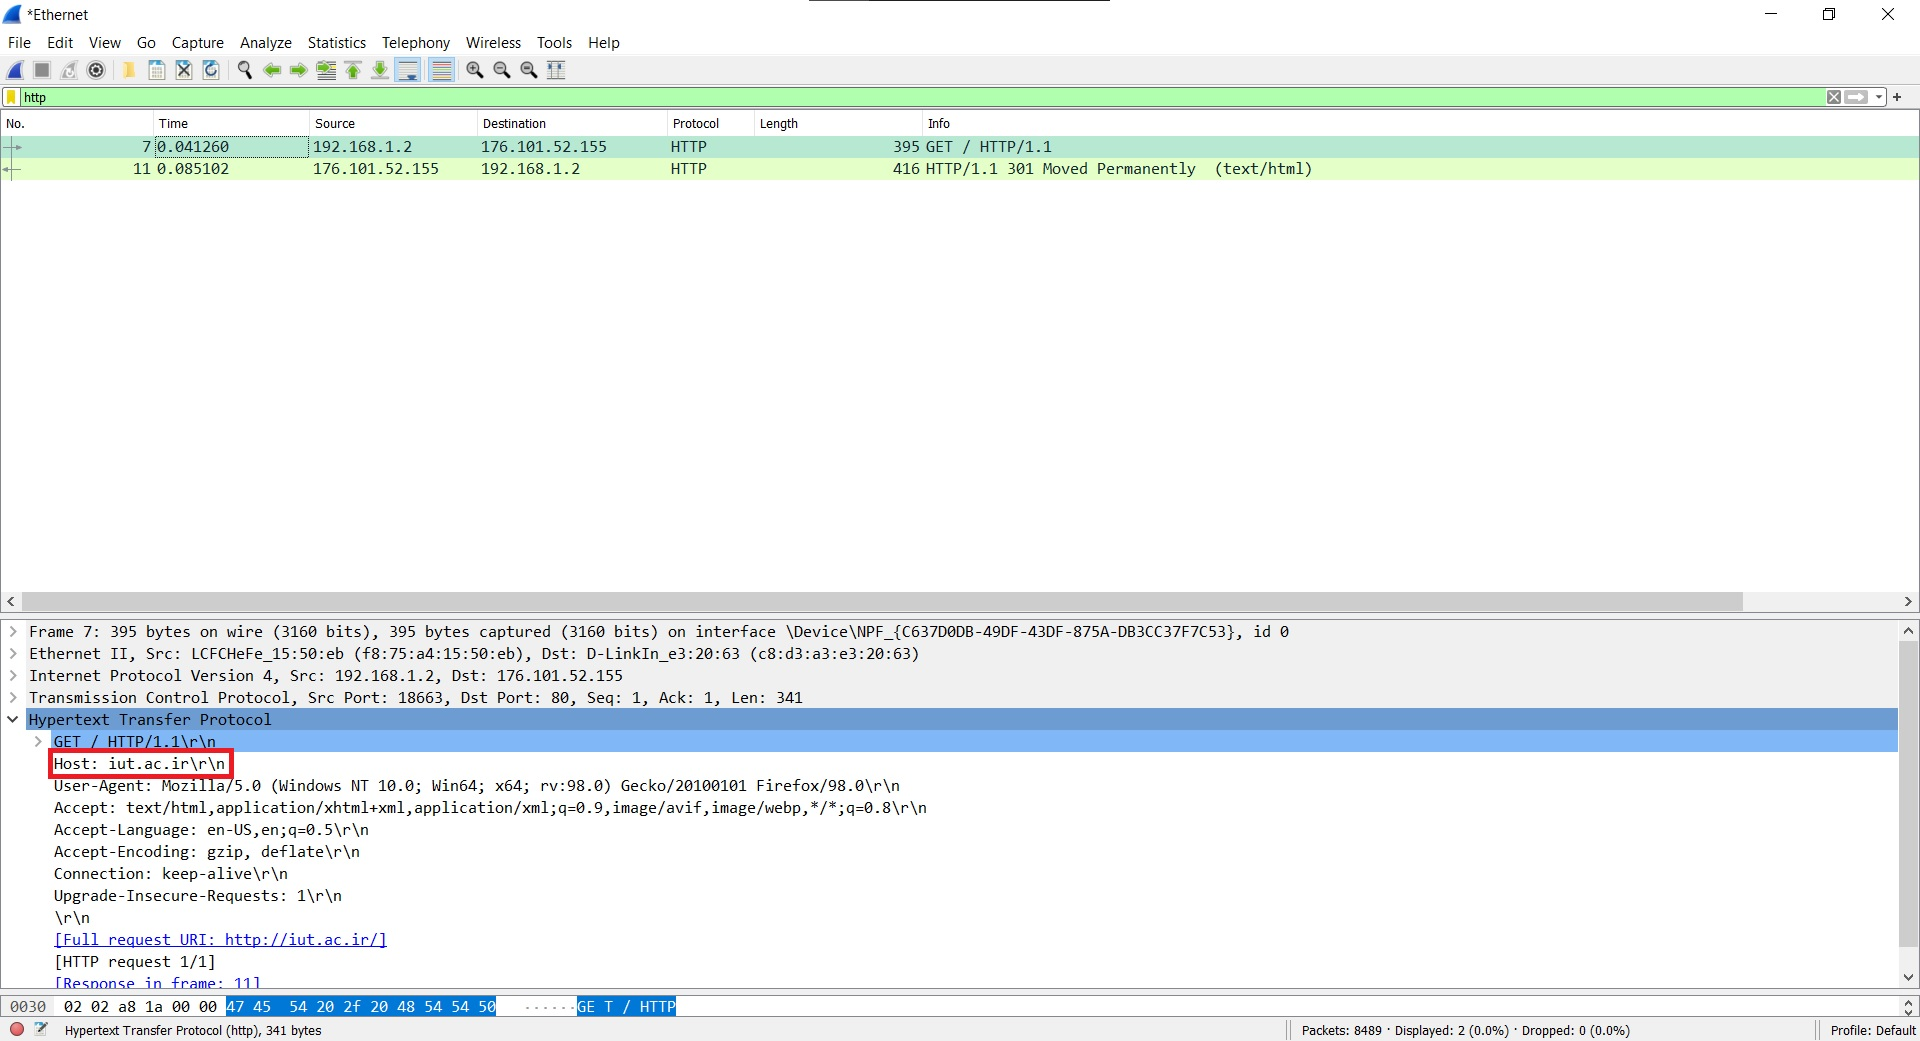
\includegraphics[width=1.0\textwidth]{figures/12.jpg}
    \caption{}
    \label{fig:fig1}
\end{figure}
\begin{figure}[H]
    \centering
    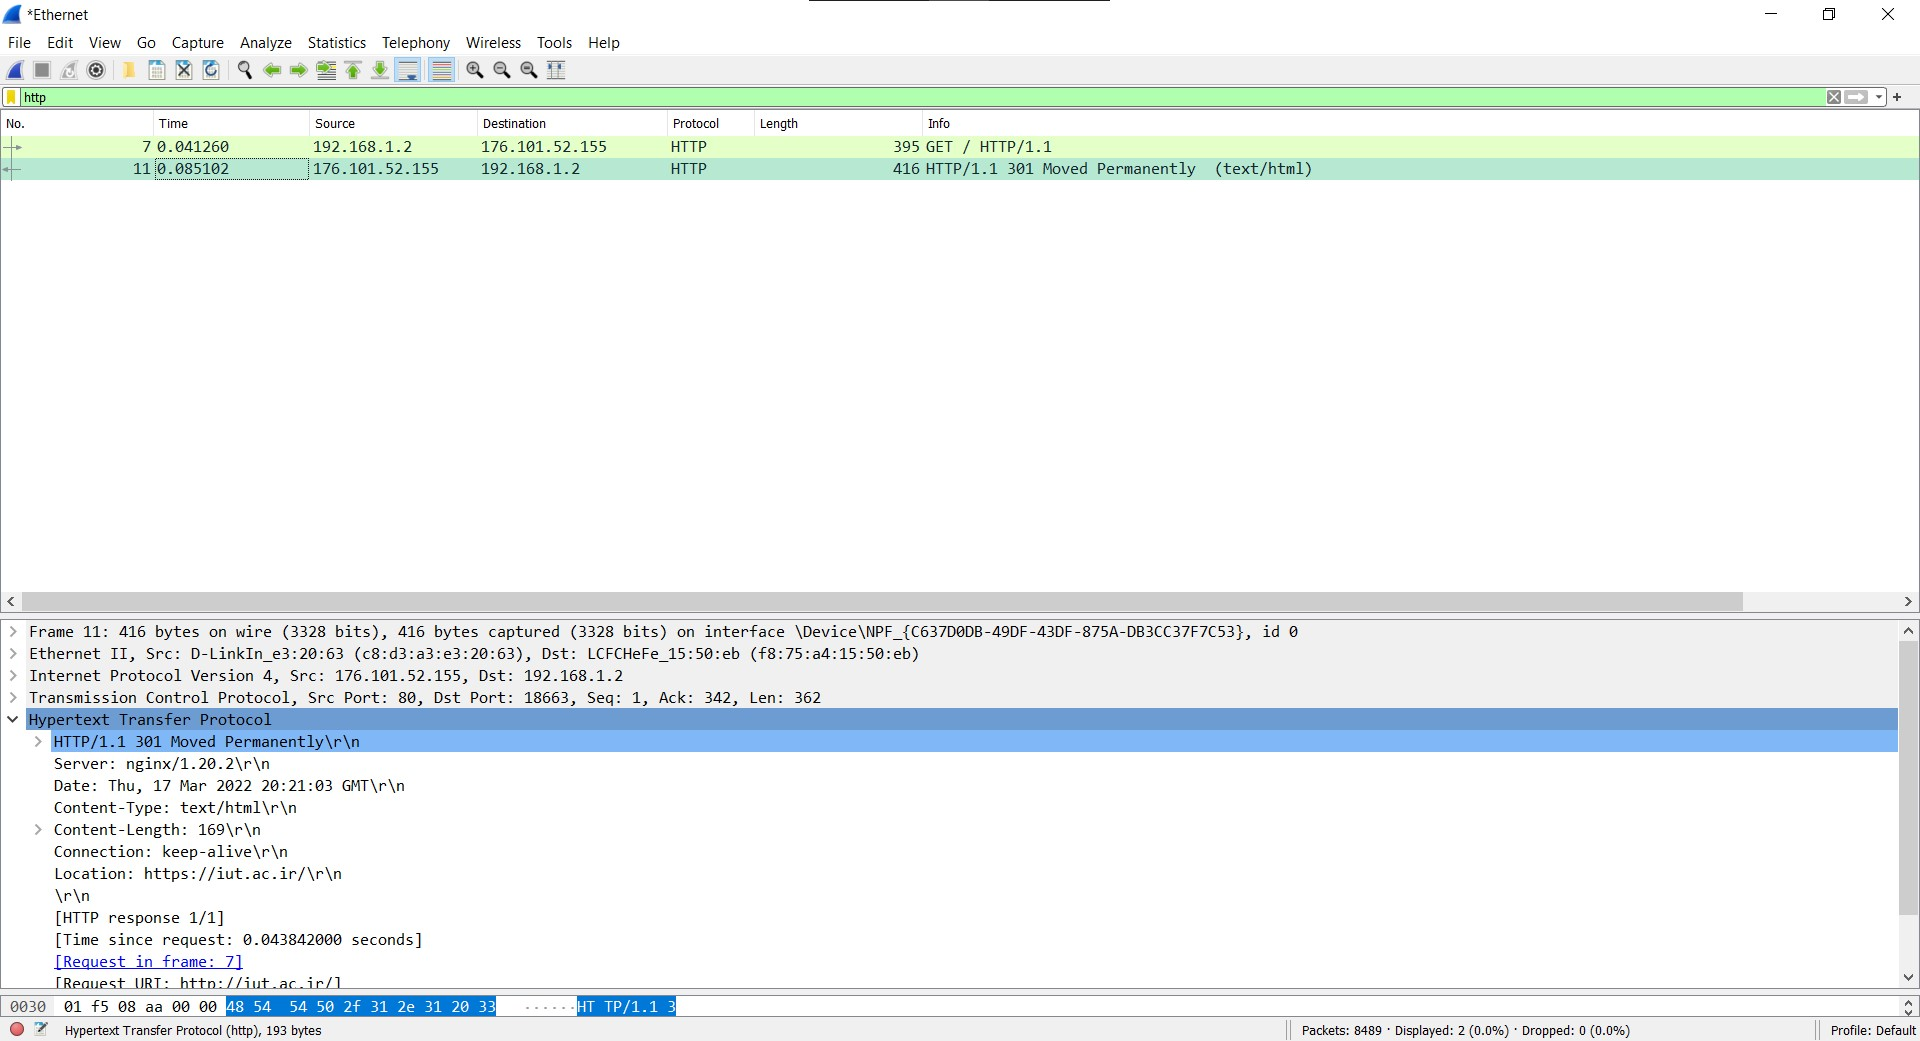
\includegraphics[width=1.0\textwidth]{figures/13.jpg}
    \caption{}
    \label{fig:fig1}
\end{figure}
\begin{figure}[H]
    \centering
    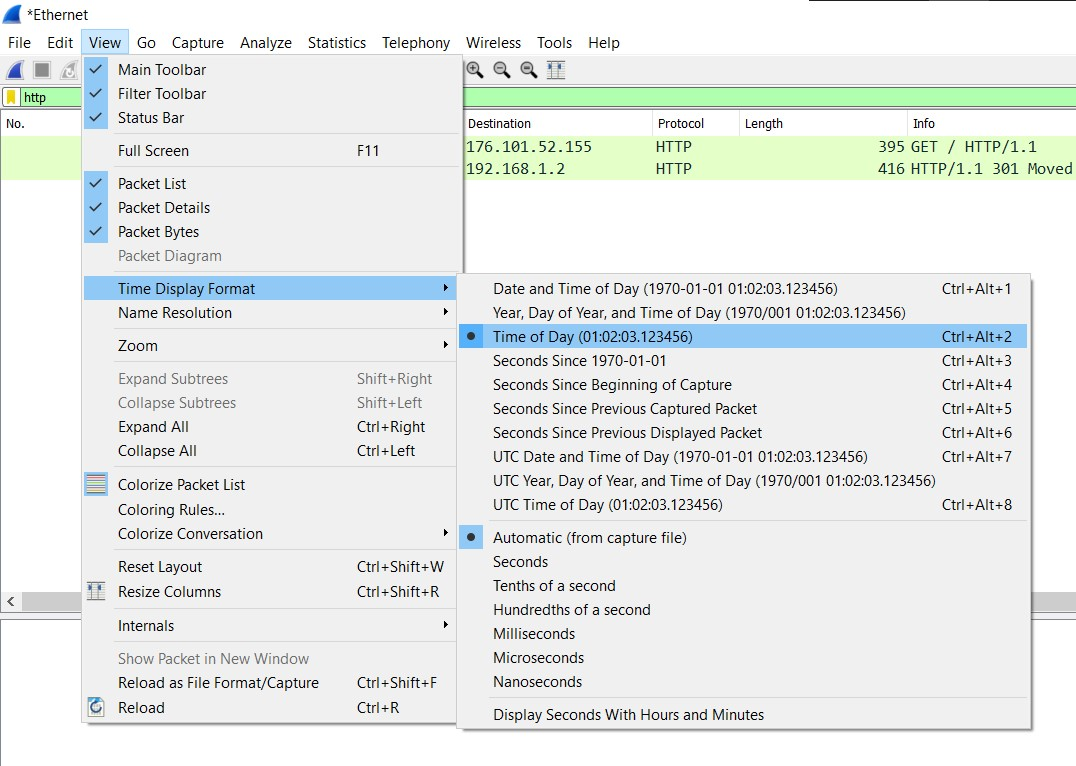
\includegraphics[width=1.0\textwidth]{figures/14.jpg}
    \caption{}
    \label{fig:fig1}
\end{figure}
\begin{figure}[H]
    \centering
    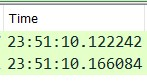
\includegraphics[width=0.5\textwidth]{figures/15.jpg}
    \caption{}
    \label{fig:fig1}
\end{figure}
این زمان برابر است با:
\begin{latin}
$
23:51:10.166084 - 23:51:10.122242 = 0.43842 s
$
\end{latin}

\subsection{}
\begin{figure}[H]
    \centering
    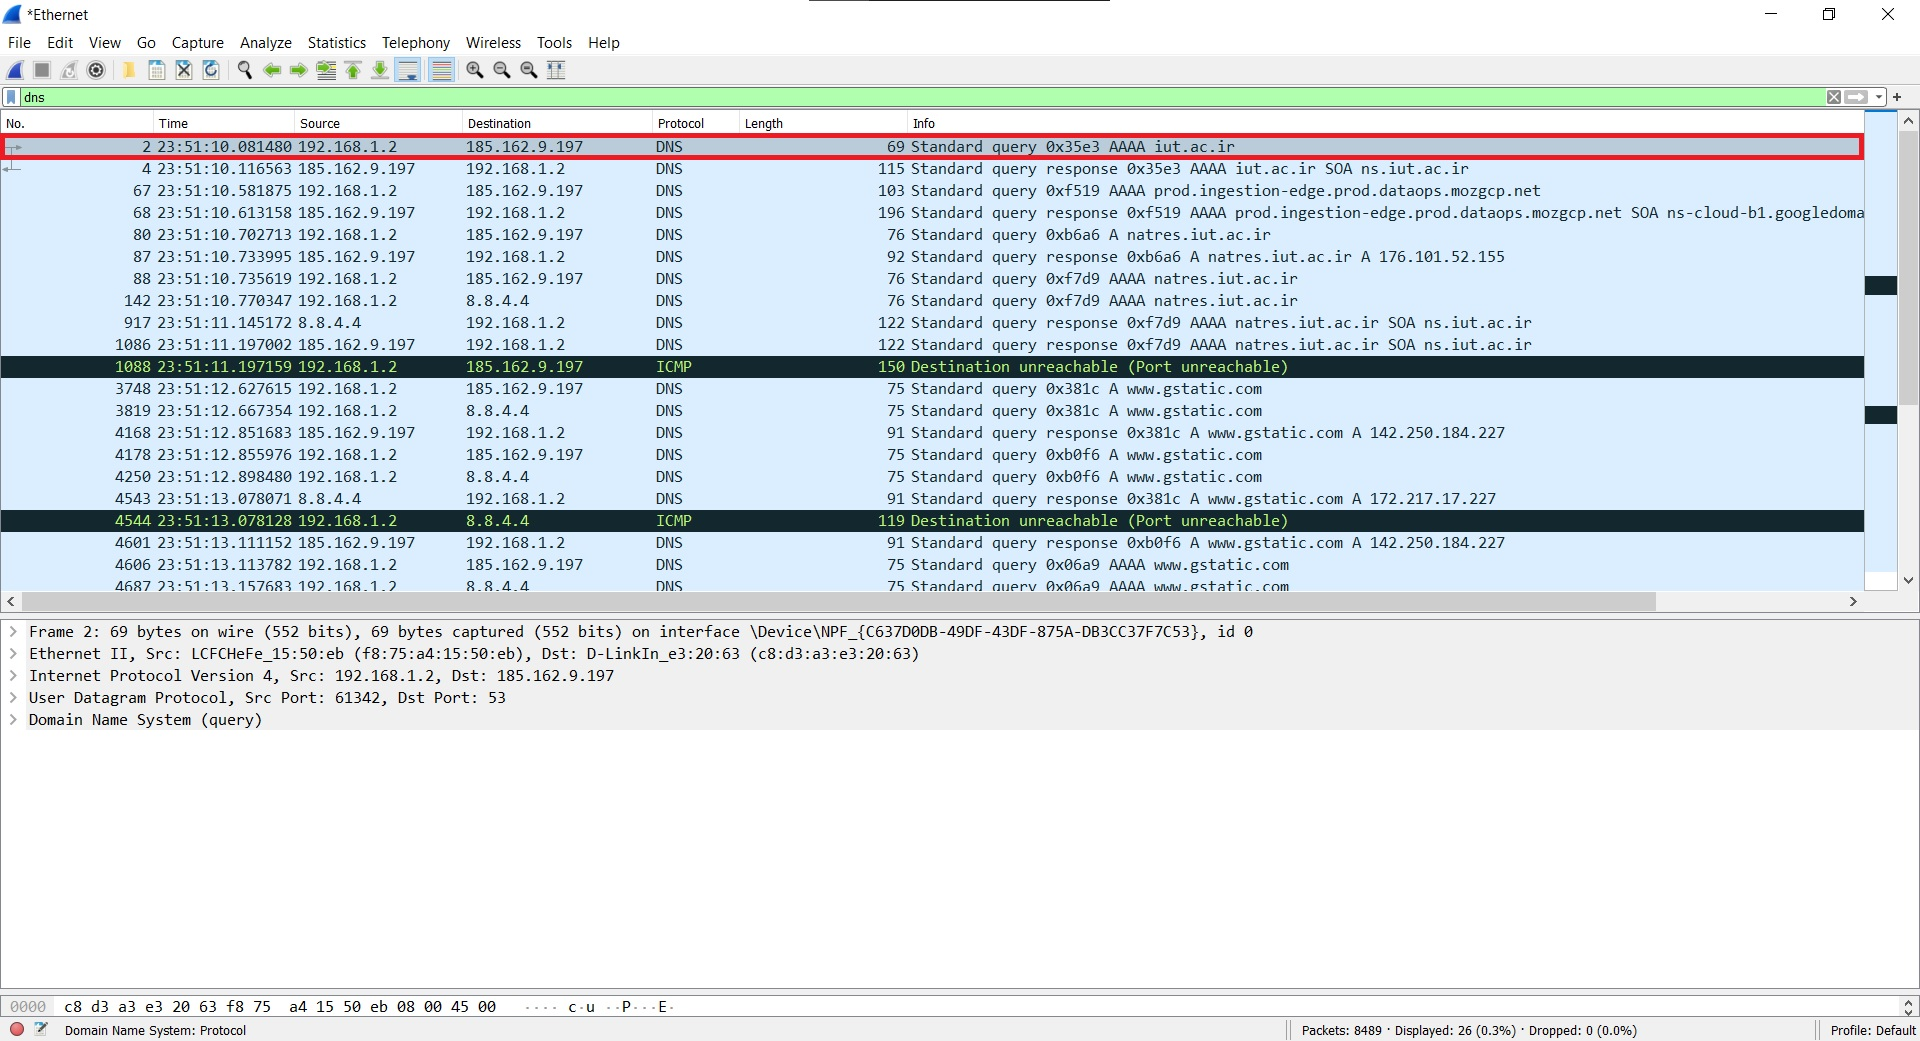
\includegraphics[width=1.0\textwidth]{figures/21.jpg}
    \caption{}
    \label{fig:fig1}
\end{figure}
\begin{figure}[H]
    \centering
    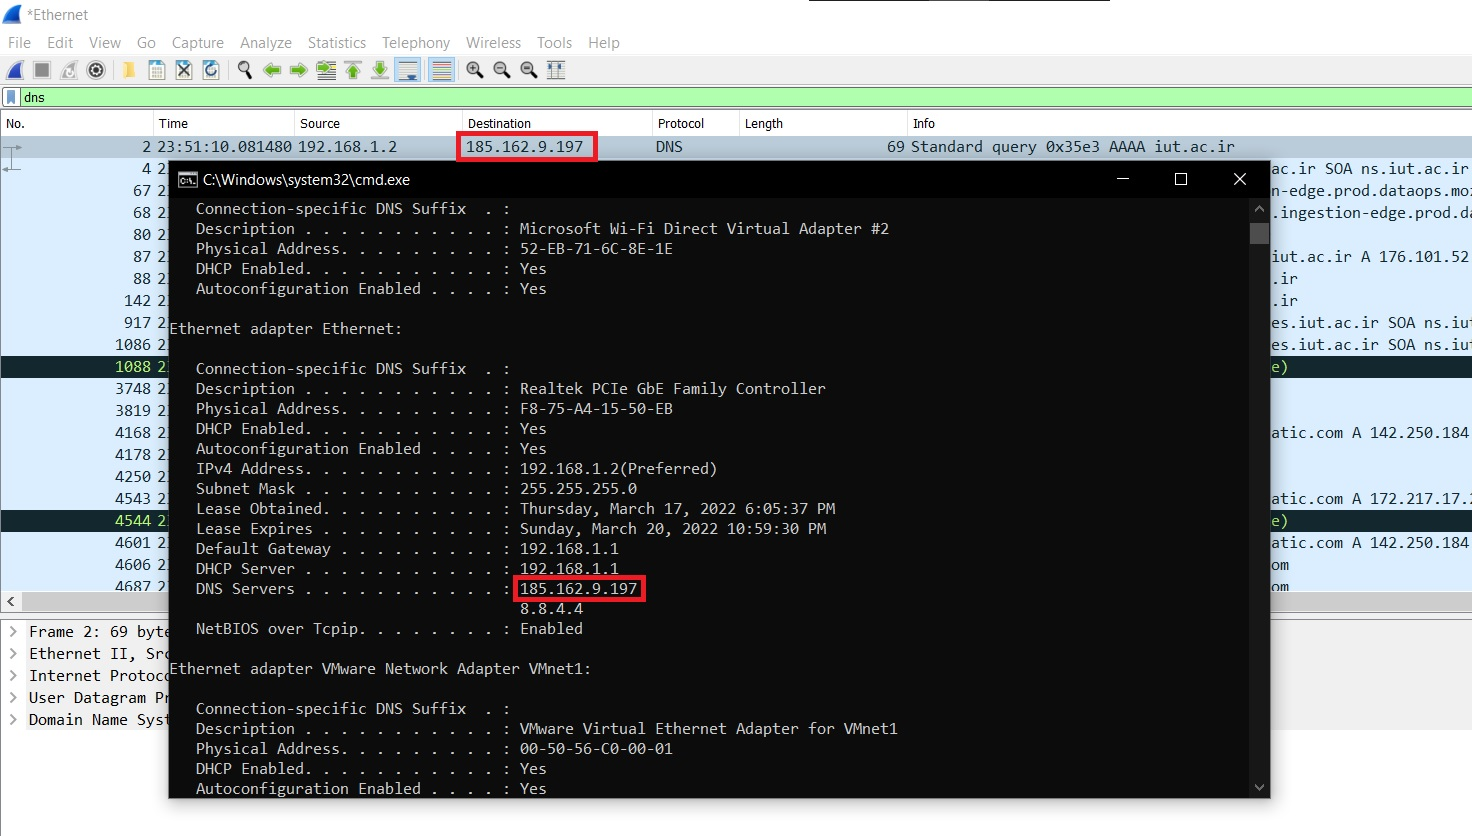
\includegraphics[width=1.0\textwidth]{figures/22.jpg}
    \caption{}
    \label{fig:fig1}
\end{figure}
آدرسِ خروجی همان آدرسِ \lr{DNS servers} متناظر با کارت شبکه در خروجی \lr{ipconfig /all} است. چون اولین کاری که برای باز کردن یک صفحه وب انجام می‌شود تبدیل آدرس سایت به آی‌پی است.


\section{}
\subsection{}
\begin{figure}[H]
    \centering
    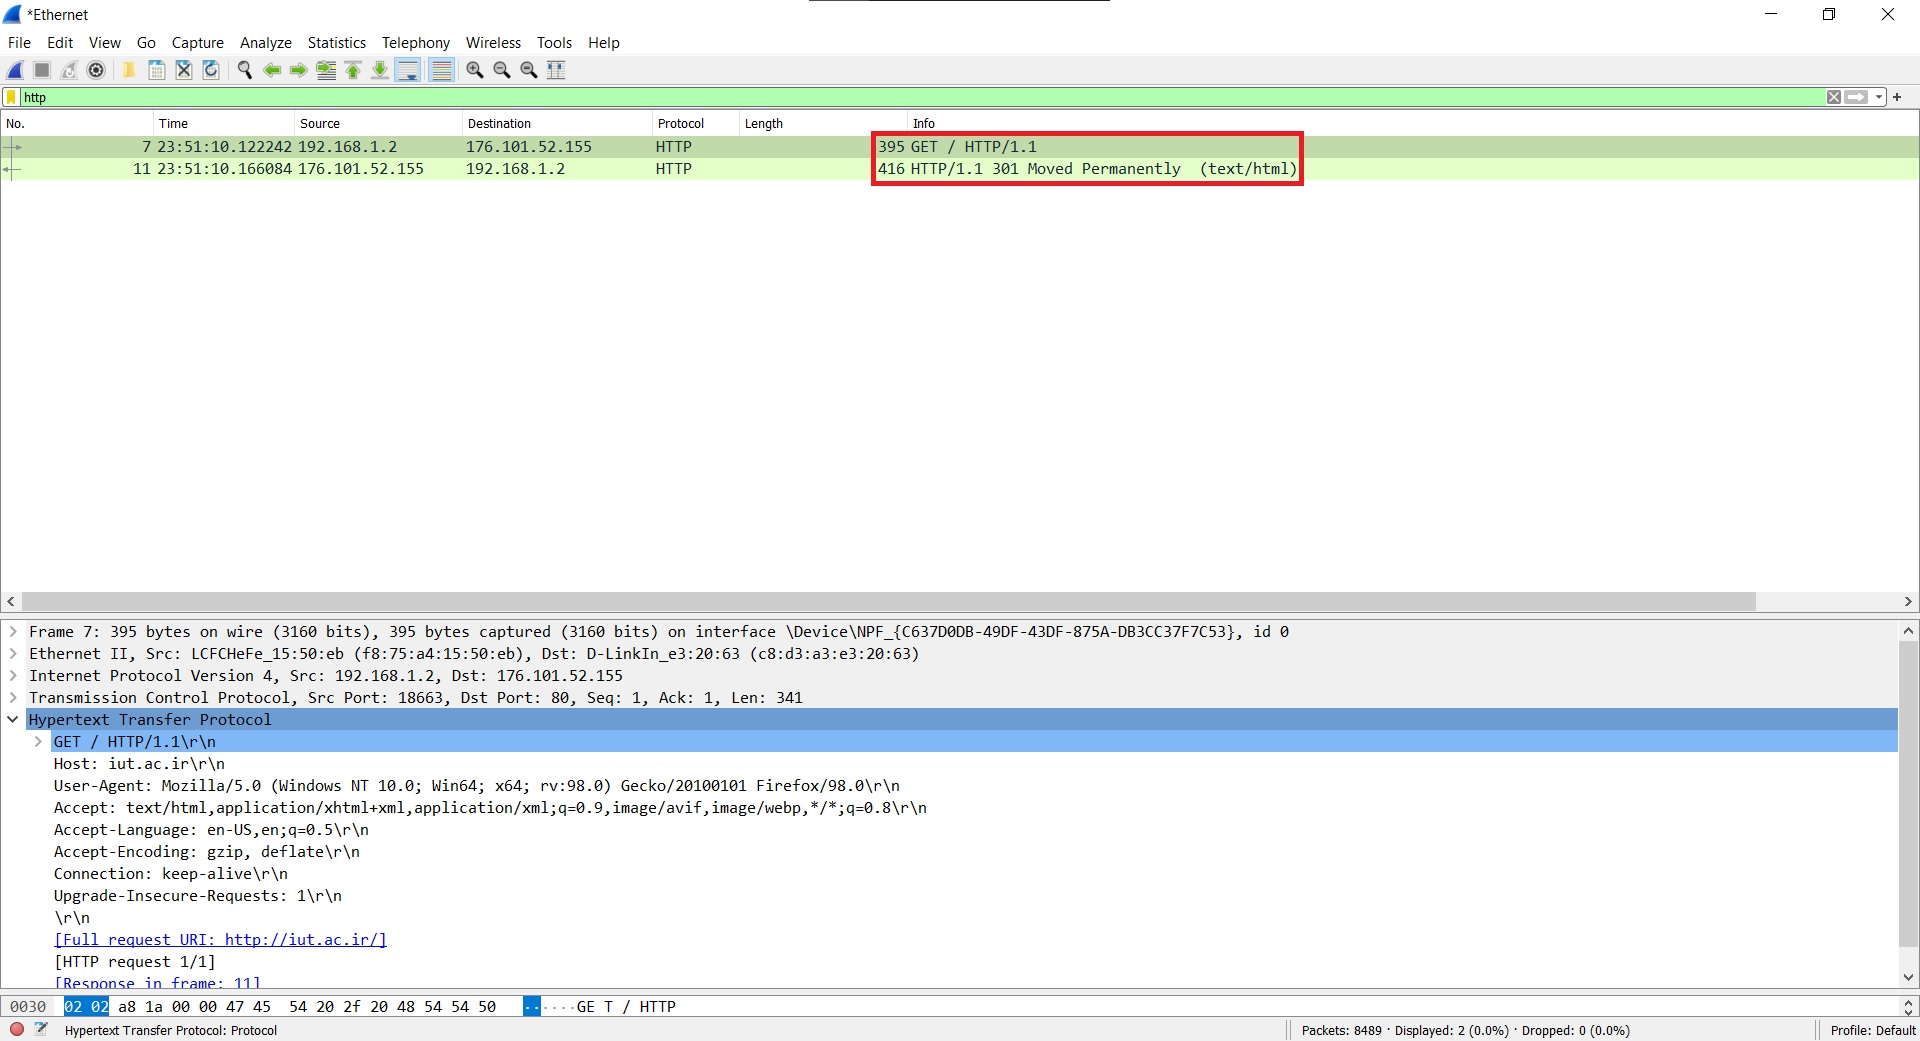
\includegraphics[width=1.0\textwidth]{figures/31.jpg}
    \caption{}
    \label{fig:fig1}
\end{figure}
هر دو 1.1 هستند (\lr{http get} متعلق به کلاینت یا همان مرورگر است). تفاوت دو نسخه در زیر شرح داده شده است:
\subsubsection{\lr{Proxy support and the Host field}}
\begin{latin}
HTTP 1.1 has a required Host header by spec.

HTTP 1.0 does not officially require a Host header, but it doesn't hurt to add one, and many applications (proxies) expect to see the Host header regardless of the protocol version.
Example:


\begin{figure}[H]
    \centering
    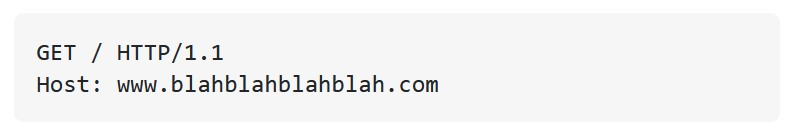
\includegraphics[width=1.0\textwidth]{figures/32.jpg}
    \caption{}
    \label{fig:fig1}
\end{figure}
This header is useful because it allows you to route a message through proxy servers, and also because your web server can distinguish between different sites on the same server.

So this means if you have blahblahlbah.com and helohelohelo.com both pointing to the same IP. Your web server can use the Host field to distinguish which site the client machine wants.
\end{latin}


\subsubsection{\lr{Persistent connections}}
\begin{latin}
HTTP 1.1 also allows you to have persistent connections which means that you can have more than one request/response on the same HTTP connection.

In HTTP 1.0 you had to open a new connection for each request/response pair. And after each response the connection would be closed. This lead to some big efficiency problems because of TCP Slow Start.
\end{latin}


\subsubsection{\lr{OPTIONS method}}
\begin{latin}
HTTP/1.1 introduces the OPTIONS method. An HTTP client can use this method to determine the abilities of the HTTP server. It's mostly used for Cross Origin Resource Sharing in web applications.
\end{latin}


\subsubsection{\lr{Caching}}
\begin{latin}
HTTP 1.0 had support for caching via the header: If-Modified-Since.

HTTP 1.1 expands on the caching support a lot by using something called 'entity tag'. If 2 resources are the same, then they will have the same entity tags.

HTTP 1.1 also adds the If-Unmodified-Since, If-Match, If-None-Match conditional headers.

There are also further additions relating to caching like the Cache-Control header. 
\end{latin}


\subsubsection{\lr{100 Continue status}}
\begin{latin}
There is a new return code in HTTP/1.1 100 Continue. This is to prevent a client from sending a large request when that client is not even sure if the server can process the request, or is authorized to process the request. In this case the client sends only the headers, and the server will tell the client 100 Continue, go ahead with the body. 
\end{latin}
\subsubsection{\lr{Much more}}
\begin{itemize}
	\item [$\bullet$] \lr{Digest authentication and proxy authentication}
	\item [$\bullet$] \lr{Extra new status codes}
	\item [$\bullet$] \lr{Chunked transfer encoding}
	\item [$\bullet$] \lr{Connection header}
	\item [$\bullet$] \lr{Enhanced compression support}
	\item [$\bullet$] \lr{Much much more. }
\end{itemize}



\subsection{}
\begin{figure}[H]
    \centering
    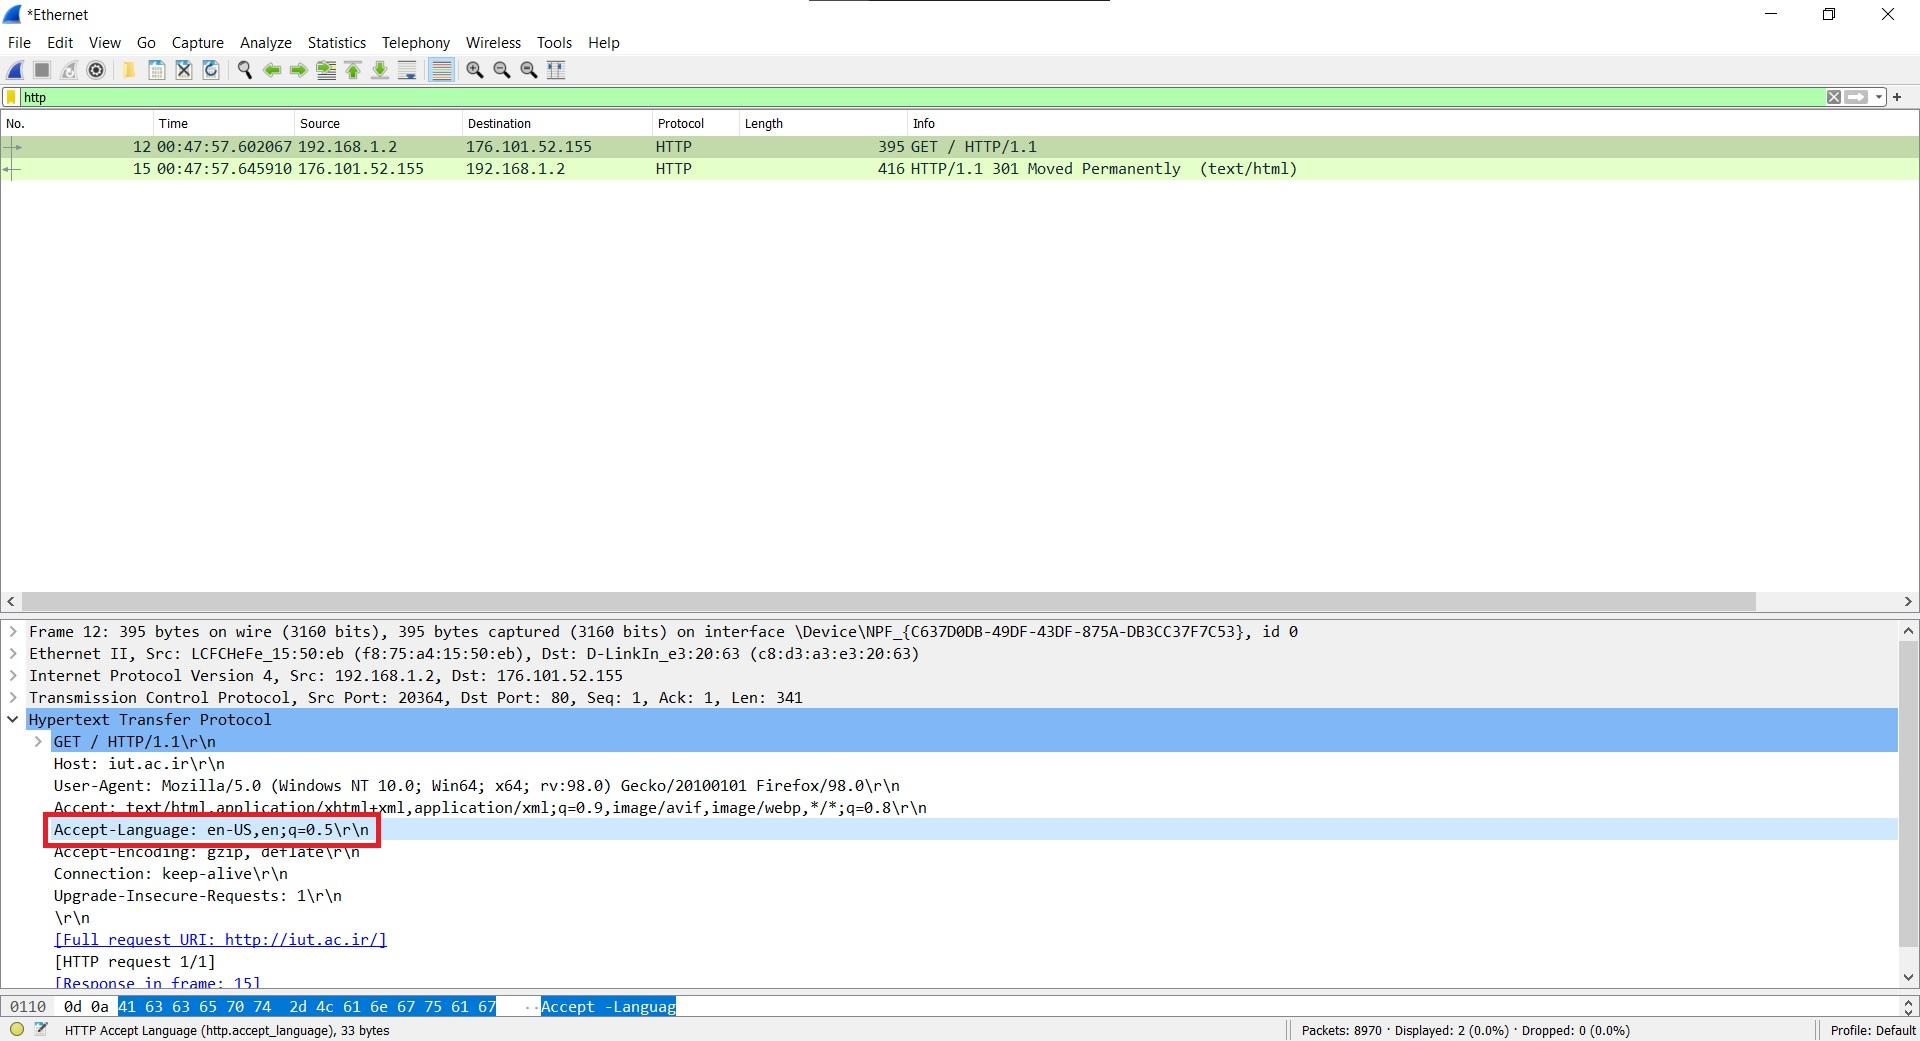
\includegraphics[width=1.0\textwidth]{figures/41.jpg}
    \caption{}
    \label{fig:fig1}
\end{figure}
تنها زبان انگلیسی از سمت مرورگر قبول است.
\subsection{}
\begin{figure}[H]
    \centering
    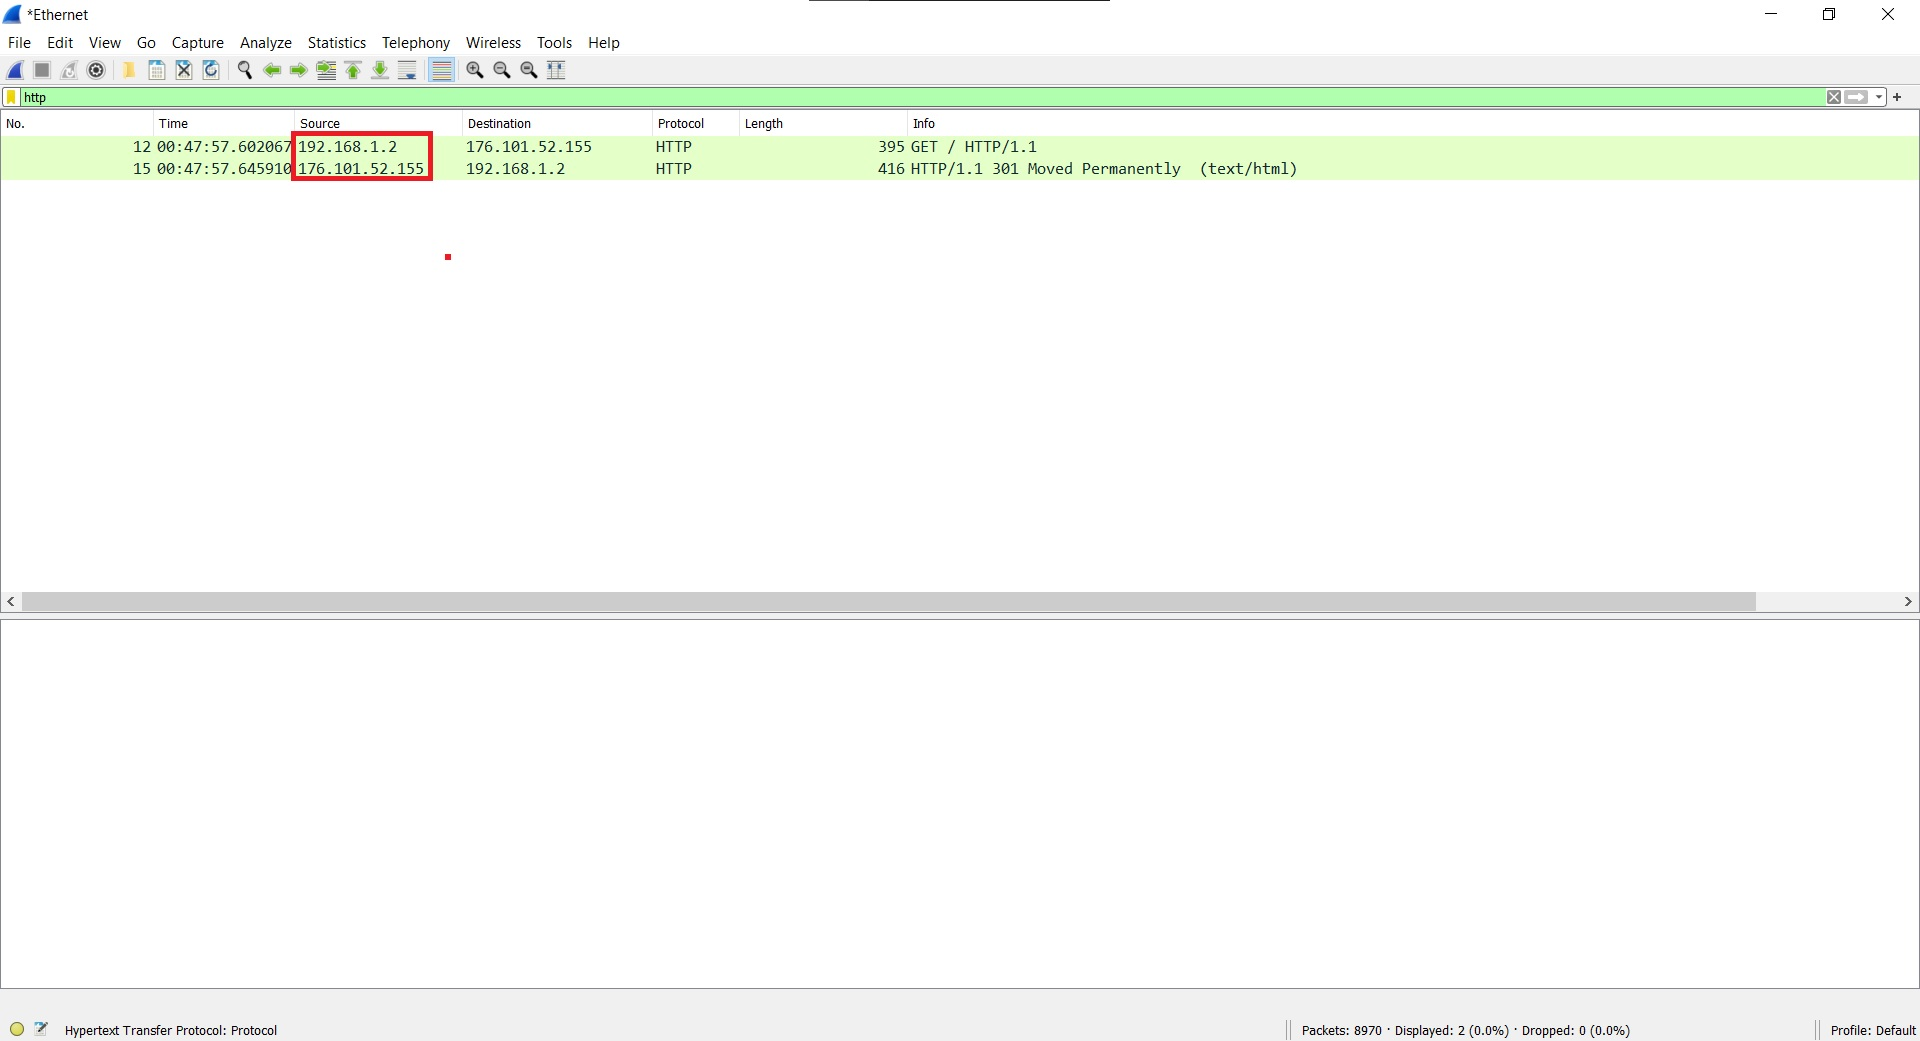
\includegraphics[width=1.0\textwidth]{figures/42.jpg}
    \caption{}
    \label{fig:fig1}
\end{figure}
آدرس آی‌پی کامپیوتر ما و سرور به ترتیب \lr{192.168.1.100} و \lr{176.101.52.155} است.
\subsection{}
\begin{figure}[H]
    \centering
    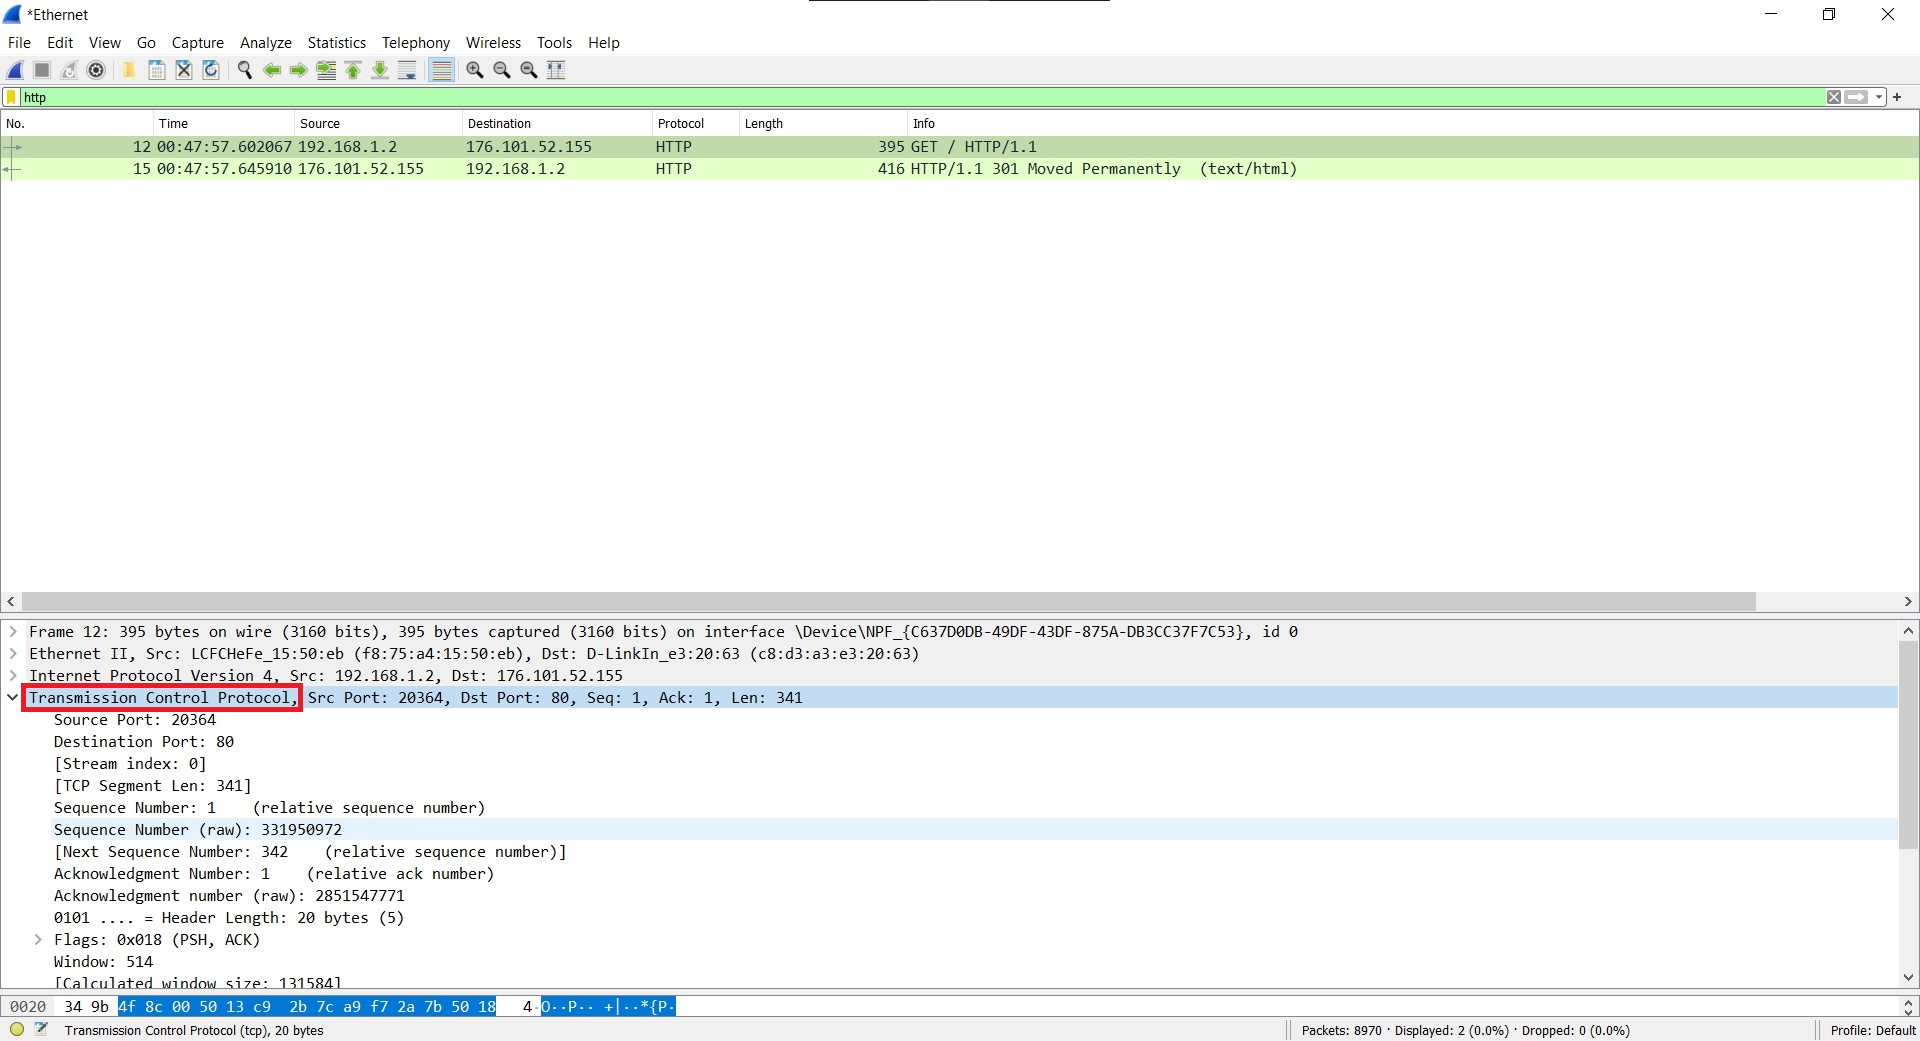
\includegraphics[width=1.0\textwidth]{figures/43.jpg}
    \caption{}
    \label{fig:fig1}
\end{figure}
از پروتکل \lr{Transmission Control Protocol(TCP)} استفاده می ‌شود.
\subsection{}
\begin{figure}[H]
    \centering
    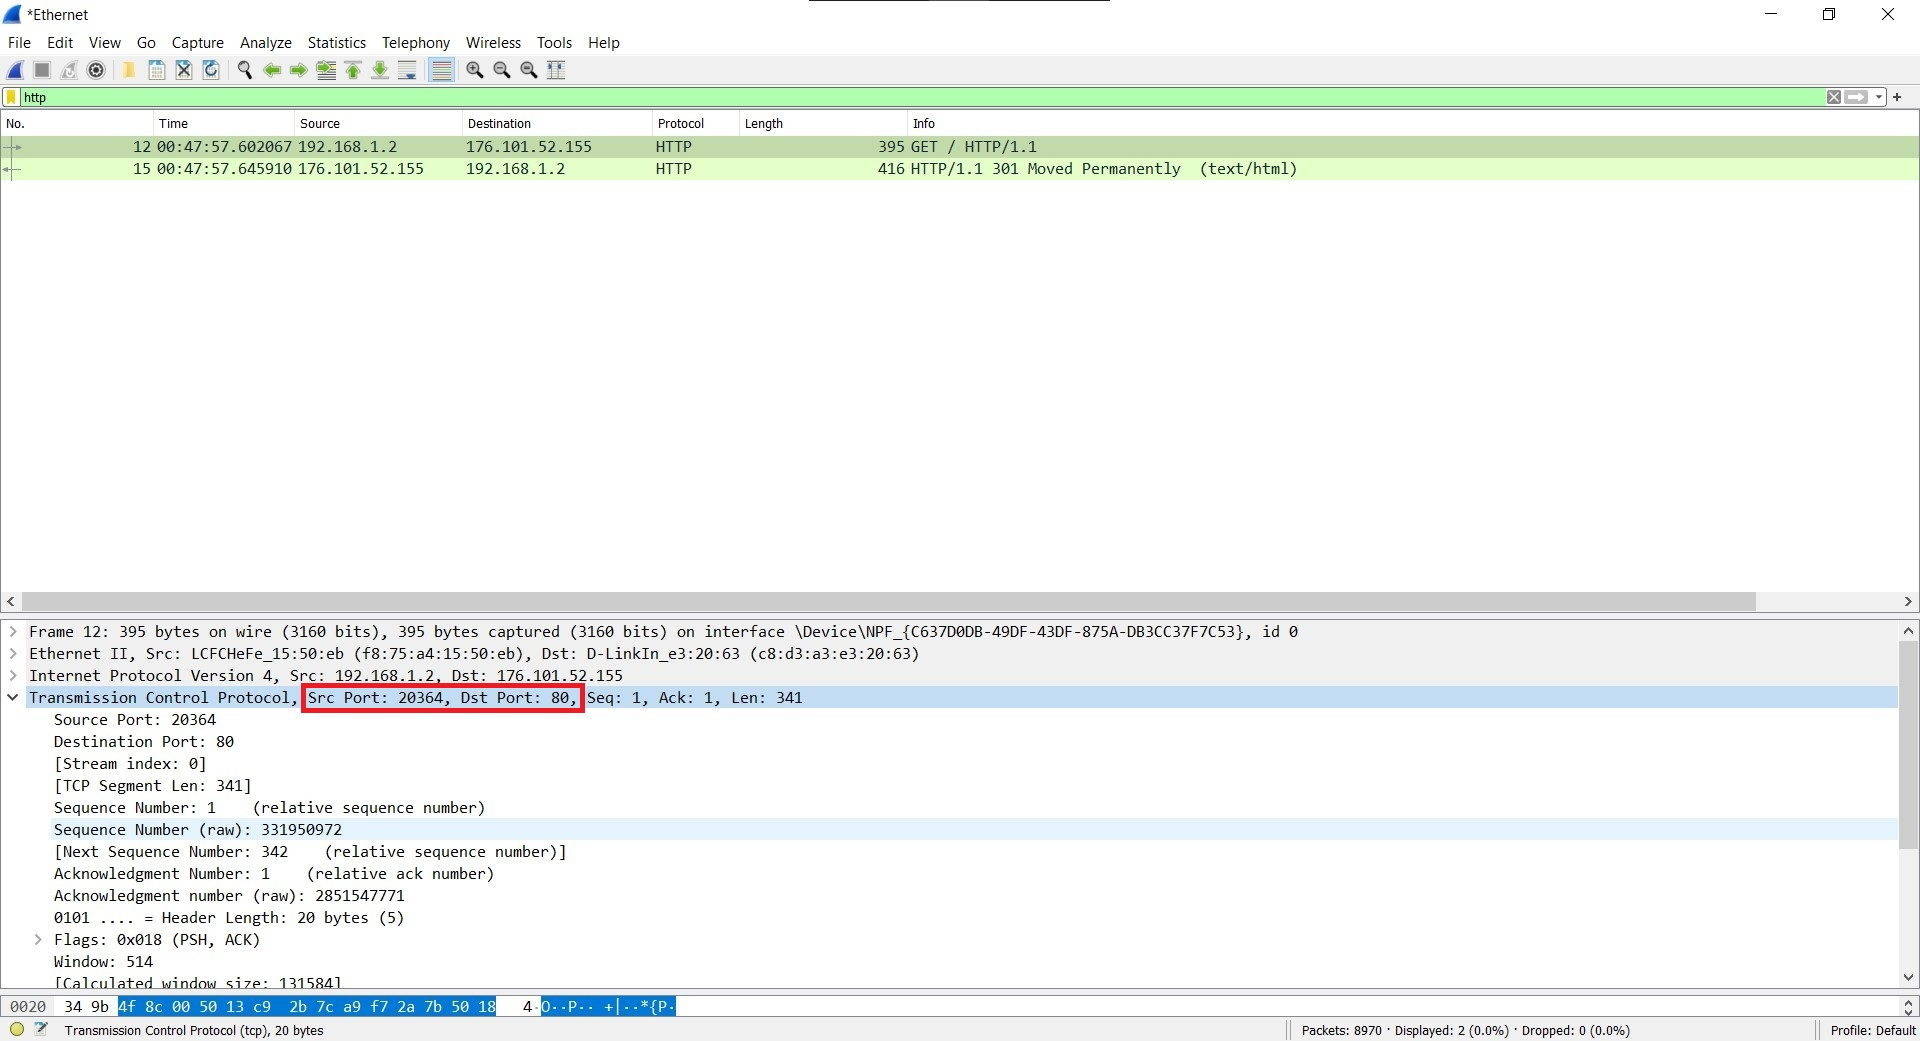
\includegraphics[width=1.0\textwidth]{figures/44.jpg}
    \caption{}
    \label{fig:fig1}
\end{figure}
چون رکورد مربوط به کلاینت را چک کردیم پس پورت مبدا و مقصد به ترتیب 20364 و 80 است.
\subsection{}
\begin{figure}[H]
    \centering
    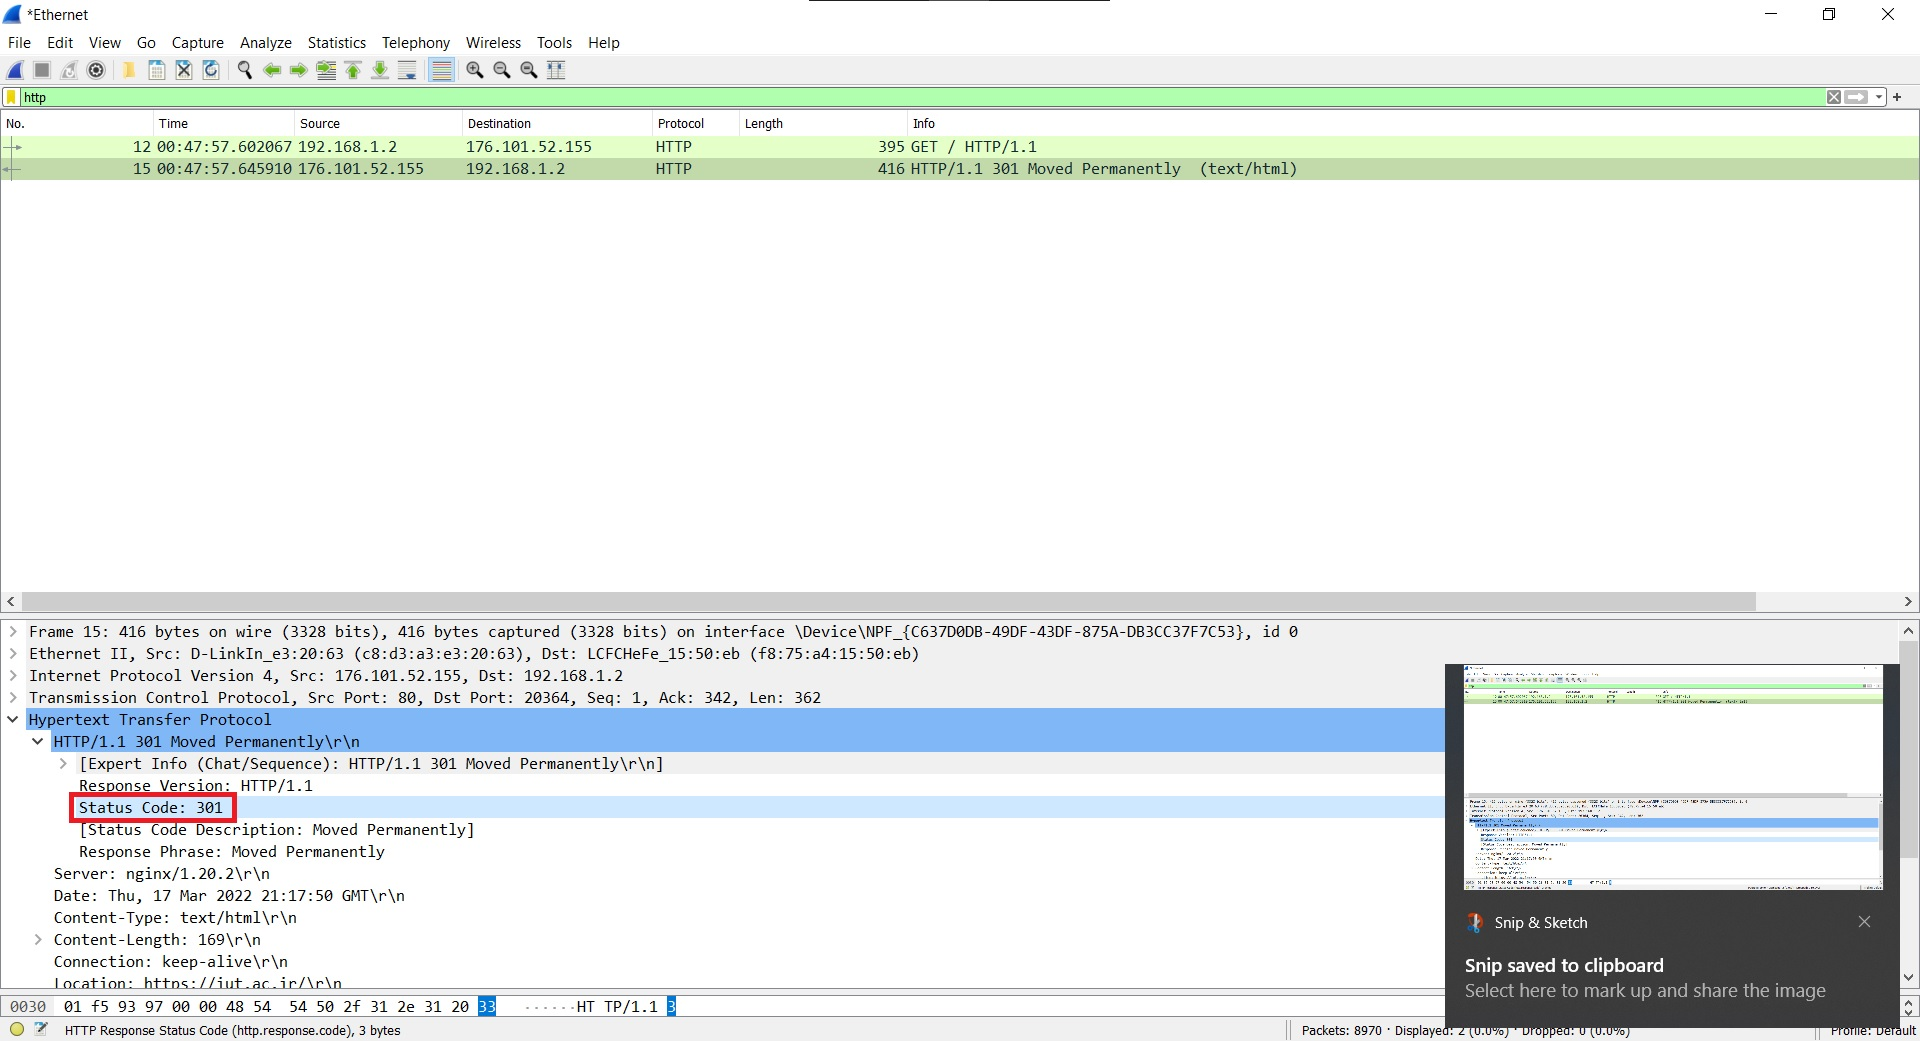
\includegraphics[width=1.0\textwidth]{figures/45.jpg}
    \caption{}
    \label{fig:fig1}
\end{figure}
کد وضعیت 301 است. کد 301،  \lr{Moved Permanently} برای تغییر مسیر دائمی استفاده می شود، به این معنی که پیوندها یا سوابق بازگرداننده این پاسخ باید به روز شوند. \lr{URL} جدید باید در قسمت \lr{Location} همراه با پاسخ ارائه شود.



\section{}
\subsection{}
\begin{figure}[H]
    \centering
    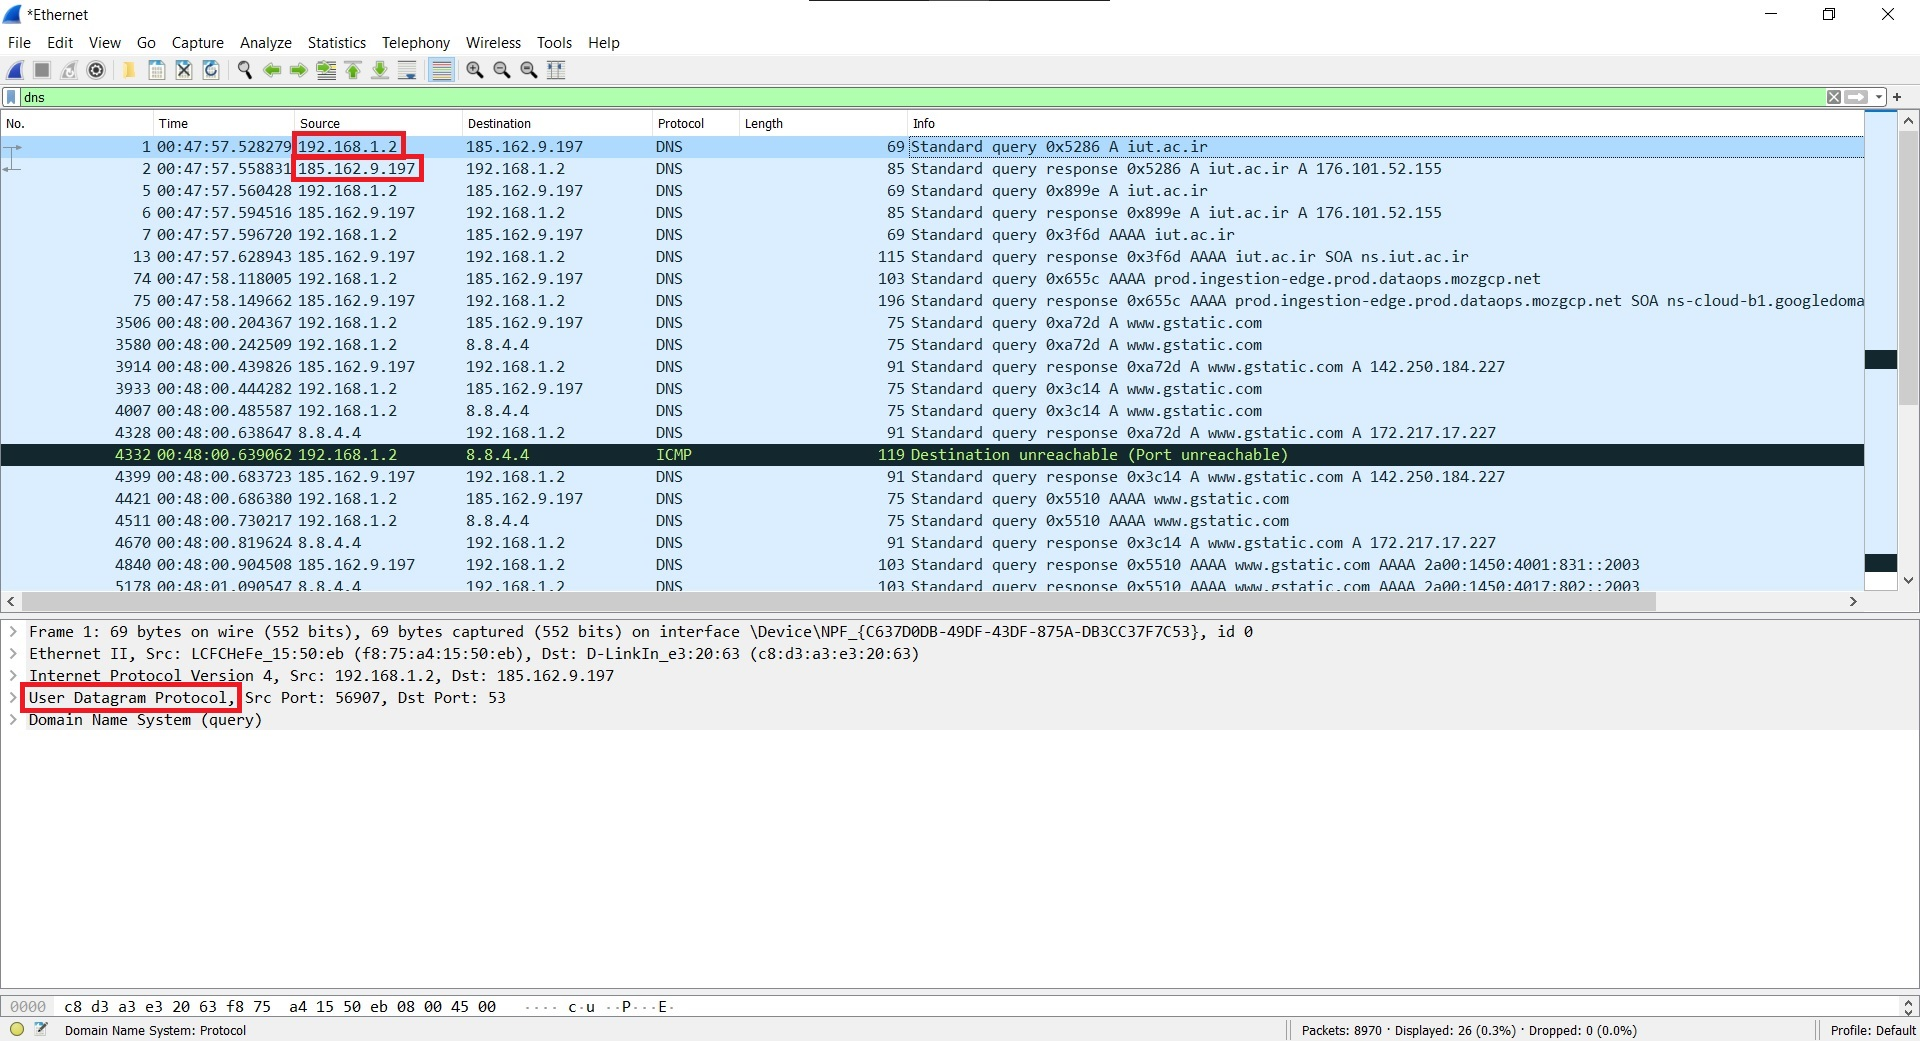
\includegraphics[width=1.0\textwidth]{figures/51.jpg}
    \caption{}
    \label{fig:fig1}
\end{figure}
آدرس فرستنده \lr{DNS query} و پیام‌های پاسخ به ترتیب برابر \lr{192.168.1.2} و \lr{185.162.9.197} است و به وسیله‌ی پروتکل \lr{UDP} فرستاده شده‌اند.
\subsection{}
\begin{figure}[H]
    \centering
    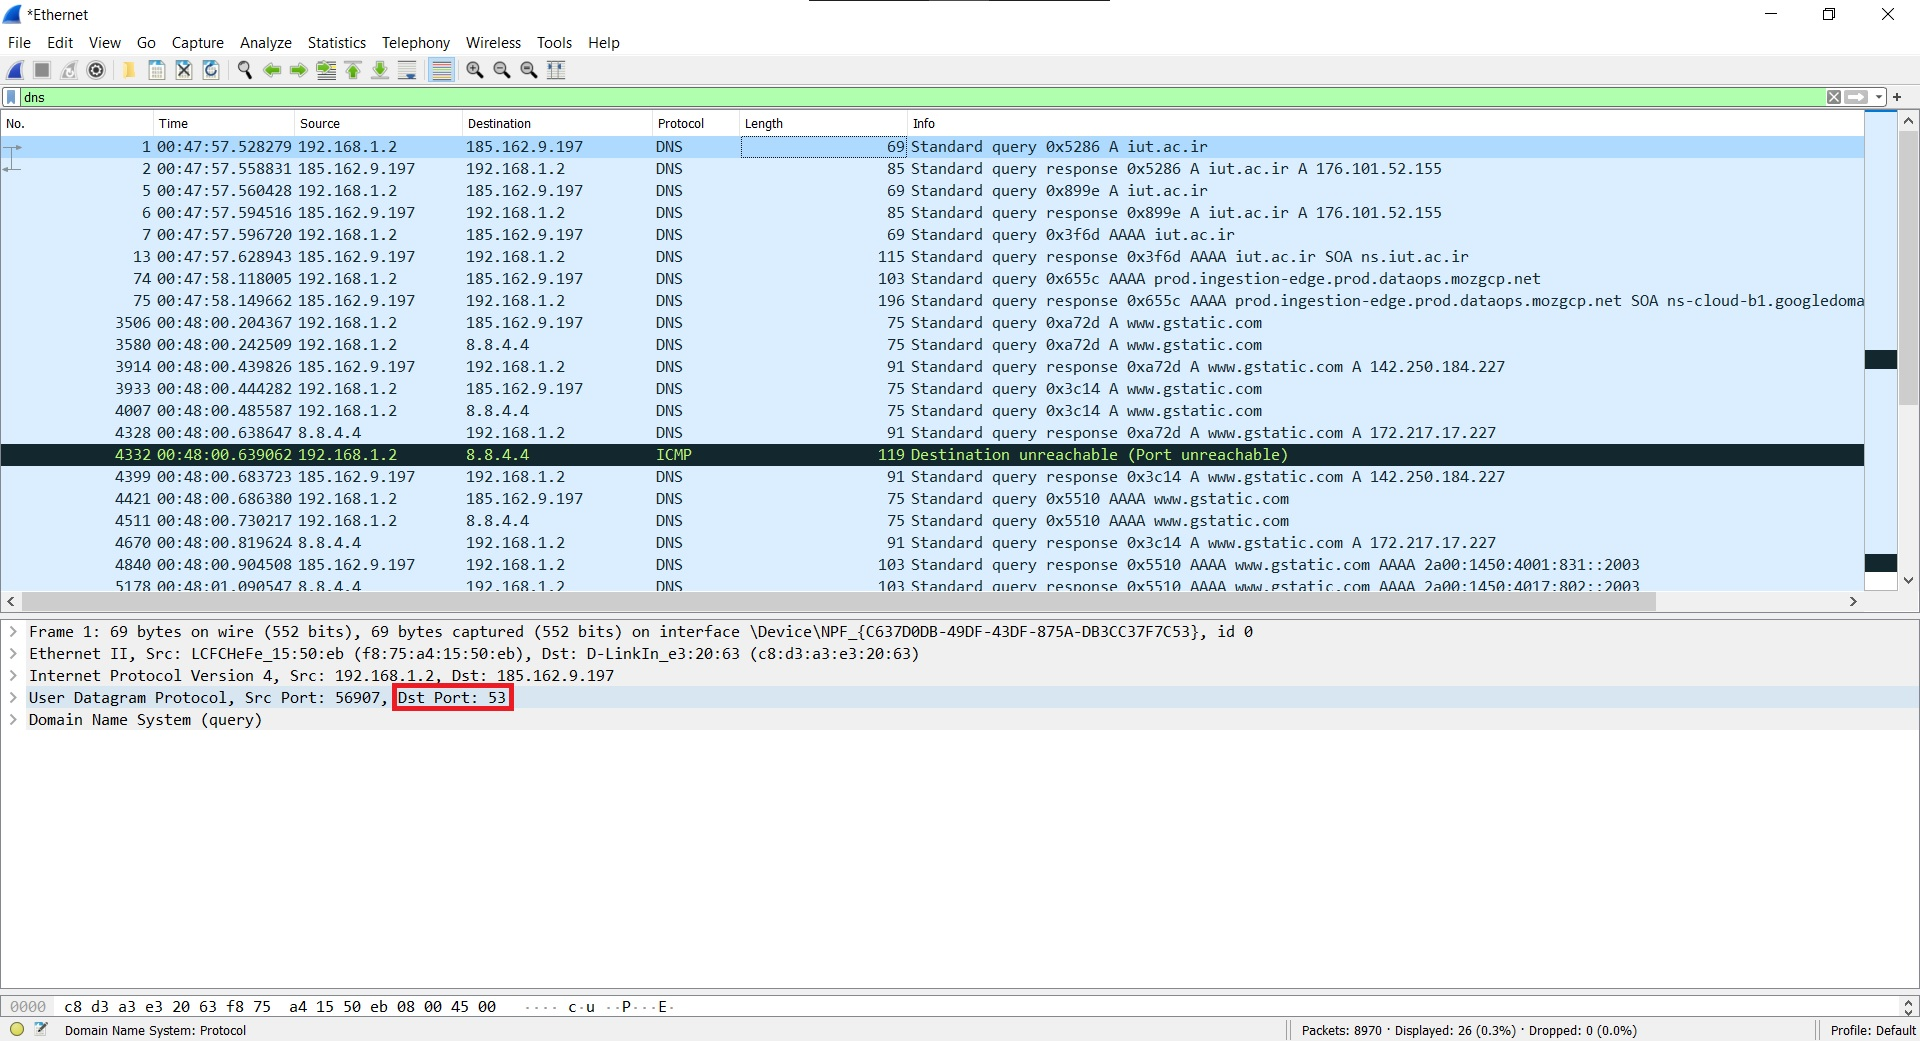
\includegraphics[width=1.0\textwidth]{figures/52.jpg}
    \caption{}
    \label{fig:fig1}
\end{figure}
\begin{figure}[H]
    \centering
    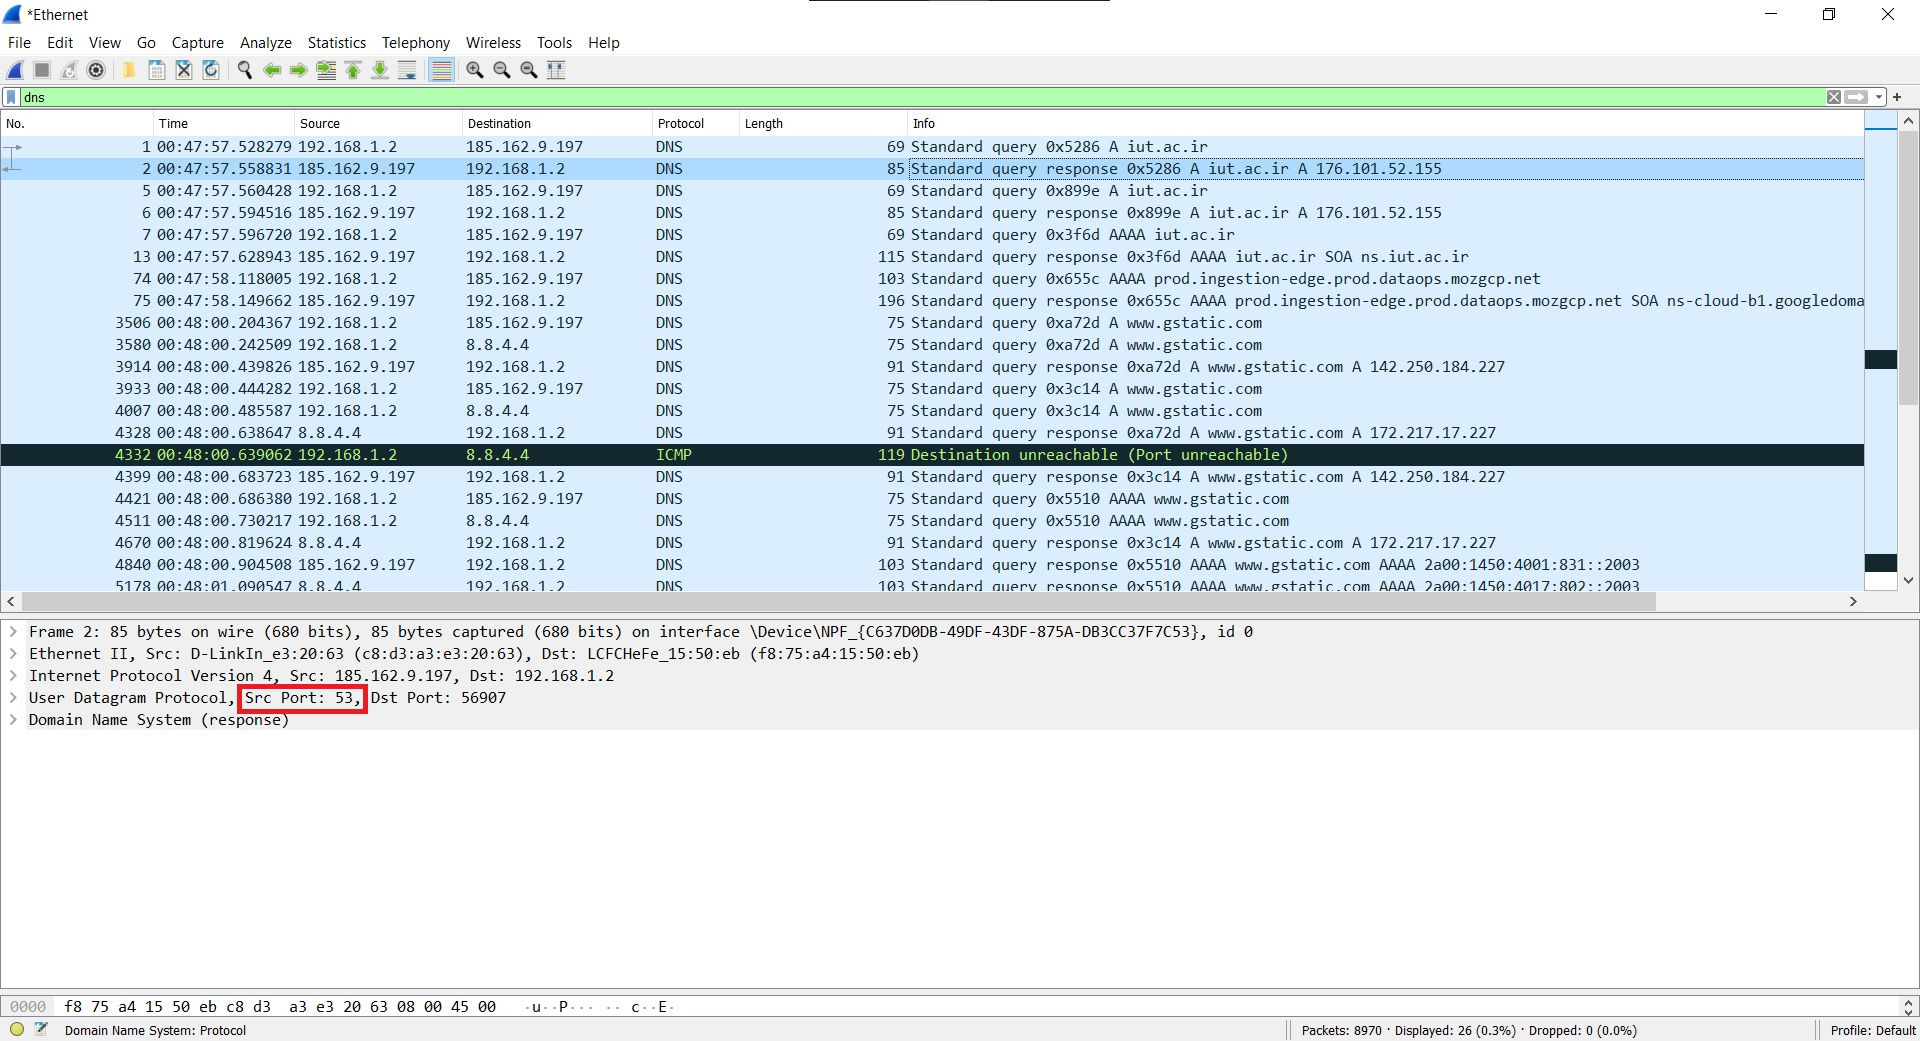
\includegraphics[width=1.0\textwidth]{figures/53.jpg}
    \caption{}
    \label{fig:fig1}
\end{figure}
شماره پورت در هر دو مورد 53 است و این به این دلیل است که \lr{DNS query} به \lr{DNS server}ِ محلی می‌رود و پاسخ آن نیز از \lr{DNS server}ِ محلی می‌آید. شماره پورت سرویس \lr{DNS} 53 است.
\subsection{}
\begin{figure}[H]
    \centering
    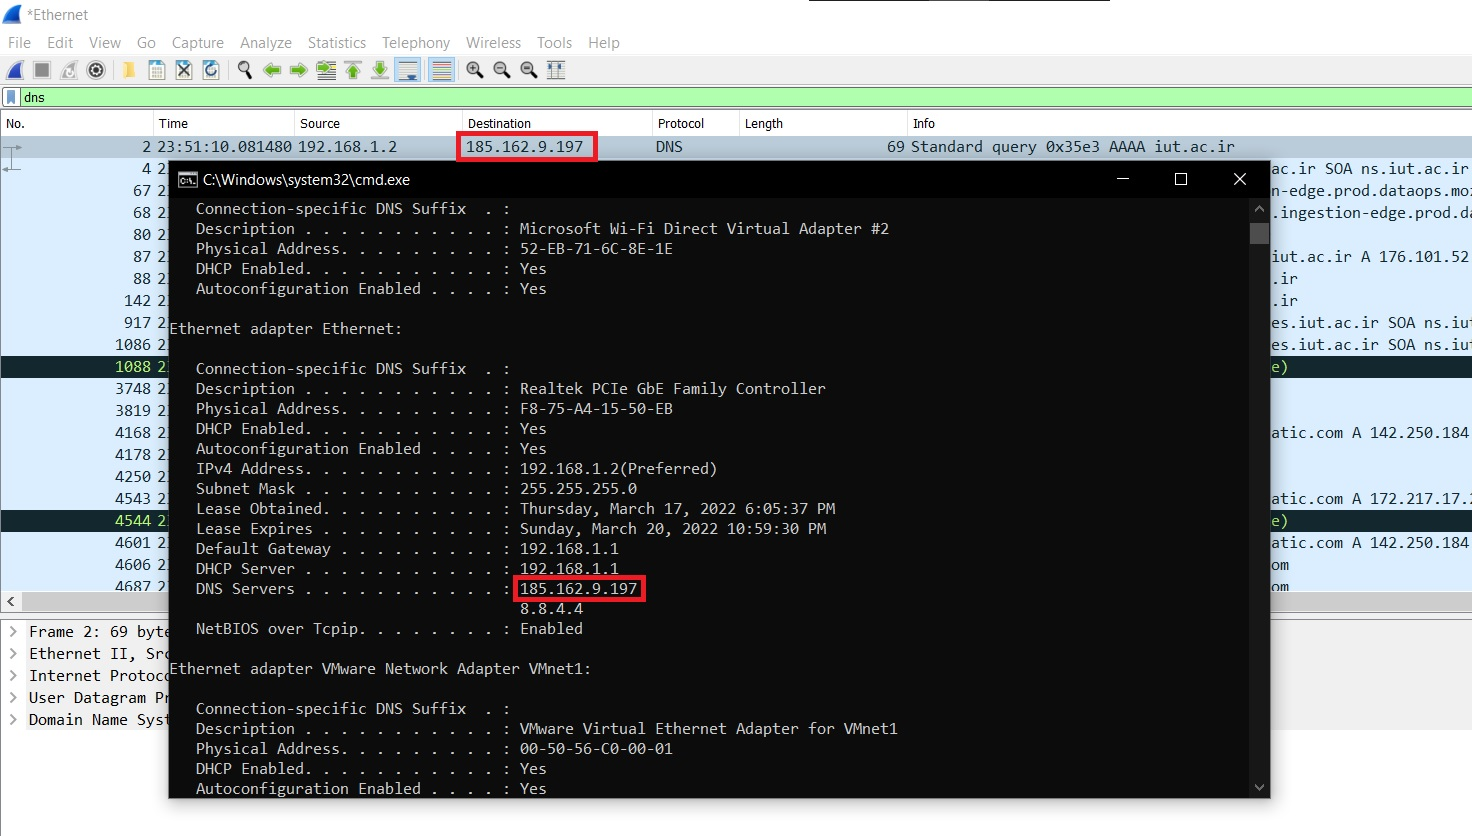
\includegraphics[width=1.0\textwidth]{figures/22.jpg}
    \caption{}
    \label{fig:fig1}
\end{figure}
همانطور که قبلا بررسی کردیم آدرسِ خروجی همان آدرسِ \lr{DNS servers} متناظر با کارت شبکه در خروجی \lr{ipconfig /all} است. چون اولین کاری که برای باز کردن یک صفحه وب انجام می‌شود تبدیل آدرس سایت به آی‌پی (سرویسِ \lr{DNS}) است.

\subsection{}
\begin{figure}[H]
    \centering
    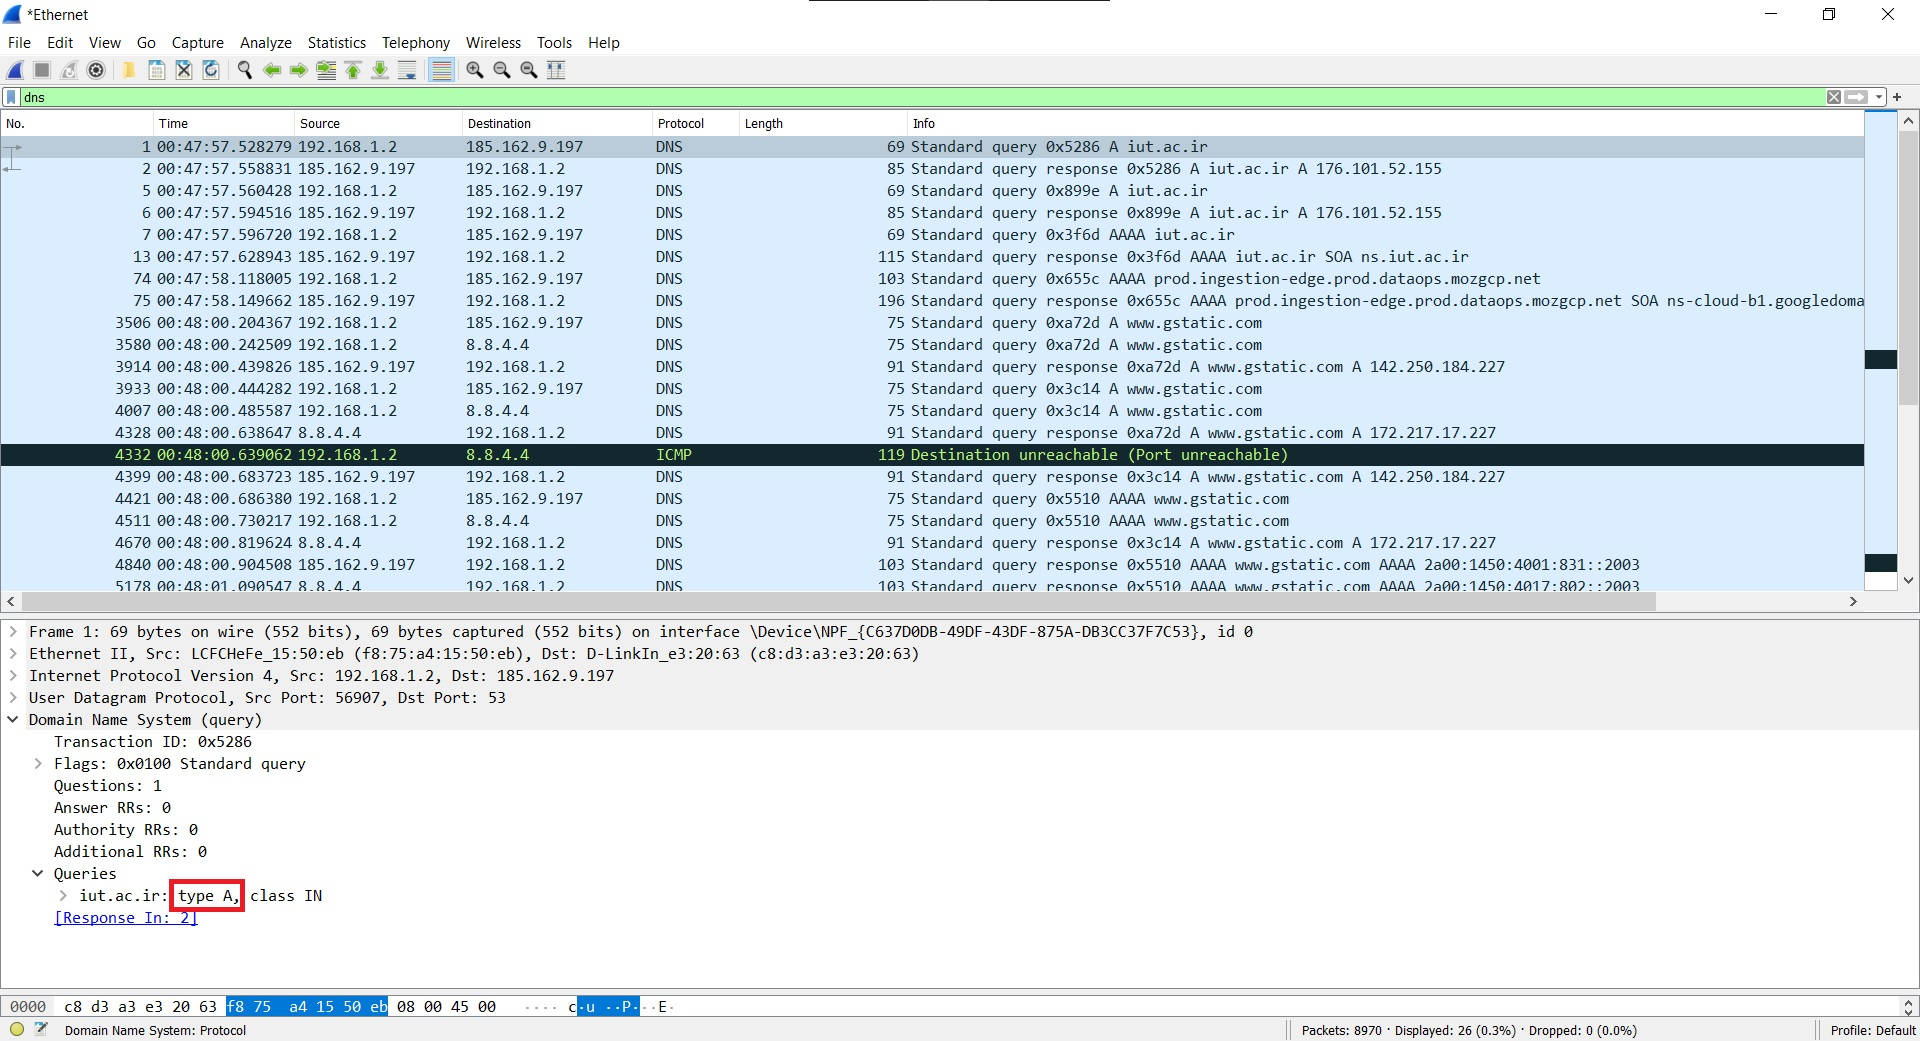
\includegraphics[width=1.0\textwidth]{figures/54.jpg}
    \caption{}
    \label{fig:fig1}
\end{figure}
نوعِ \lr{A} است و در خودش جواب ندارد.

\subsection{}
\begin{figure}[H]
    \centering
    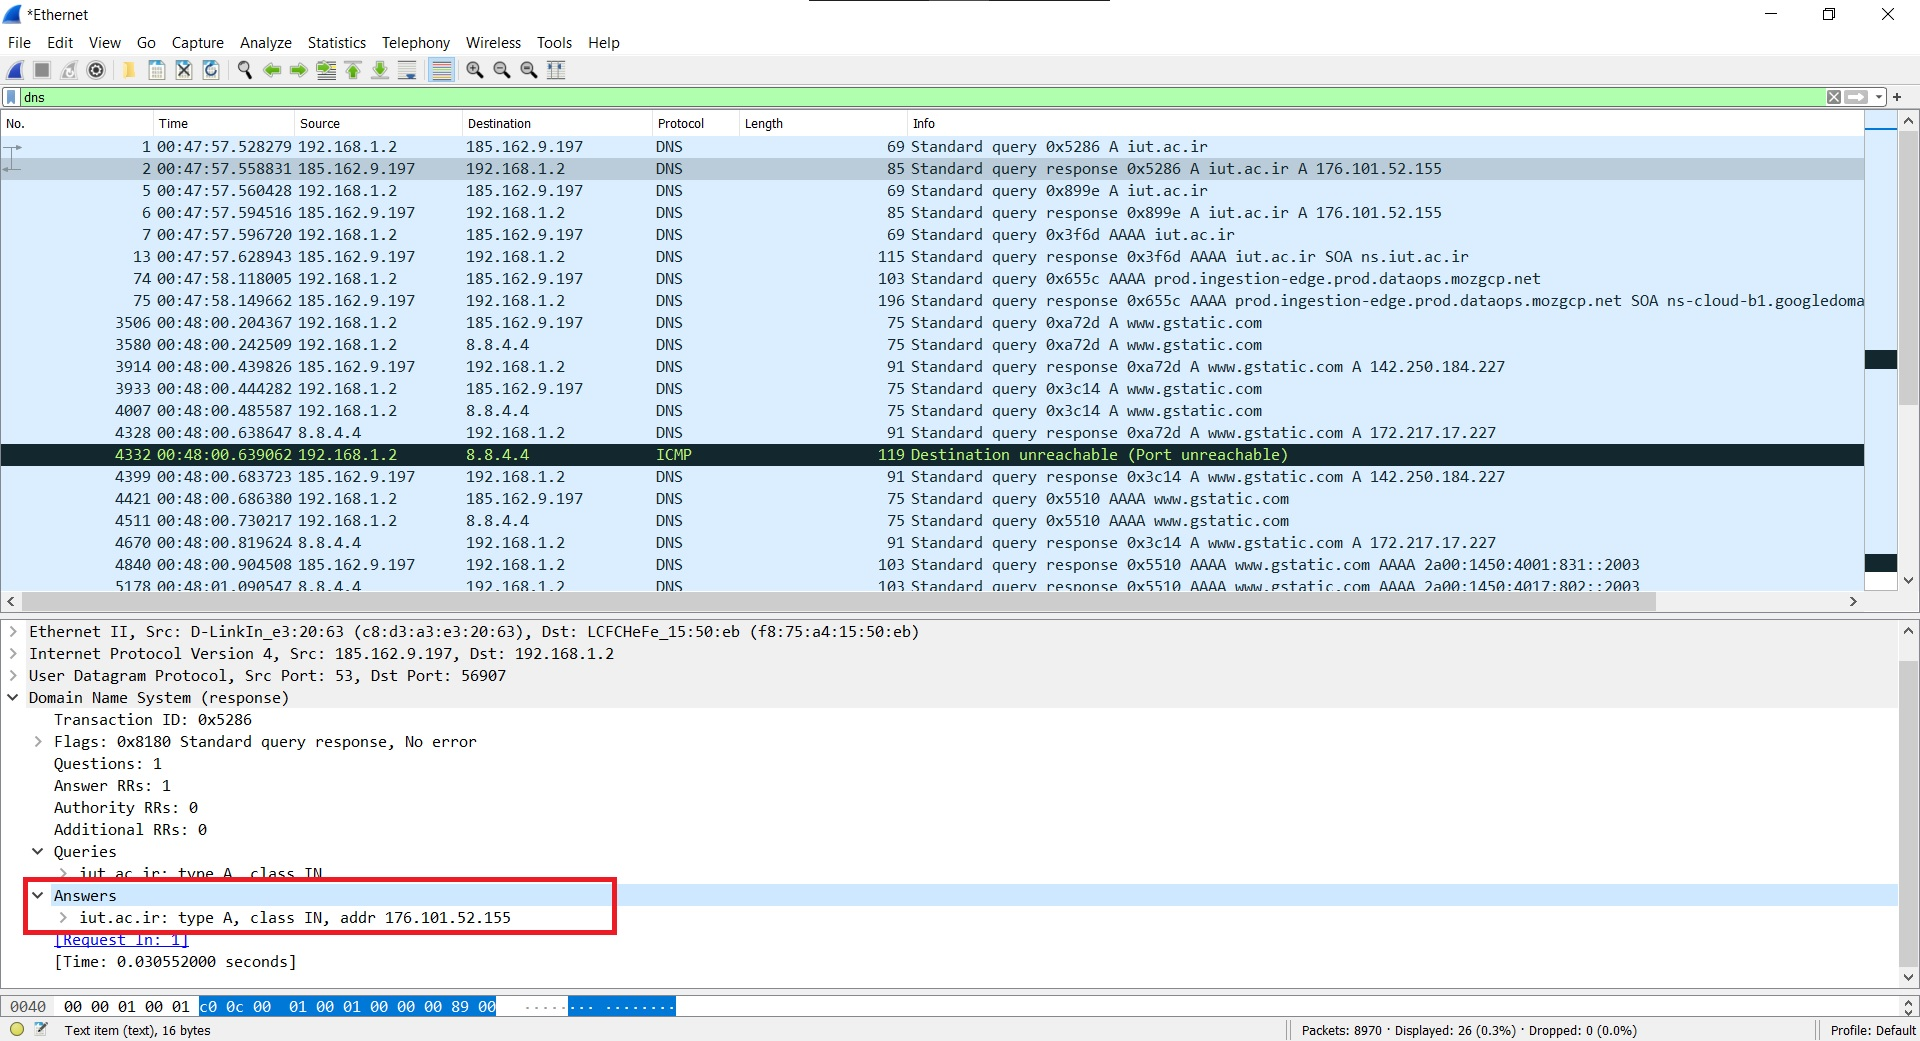
\includegraphics[width=1.0\textwidth]{figures/55.jpg}
    \caption{}
    \label{fig:fig1}
\end{figure}
فقط یک جواب دارد.
\subsection{}
\begin{figure}[H]
    \centering
    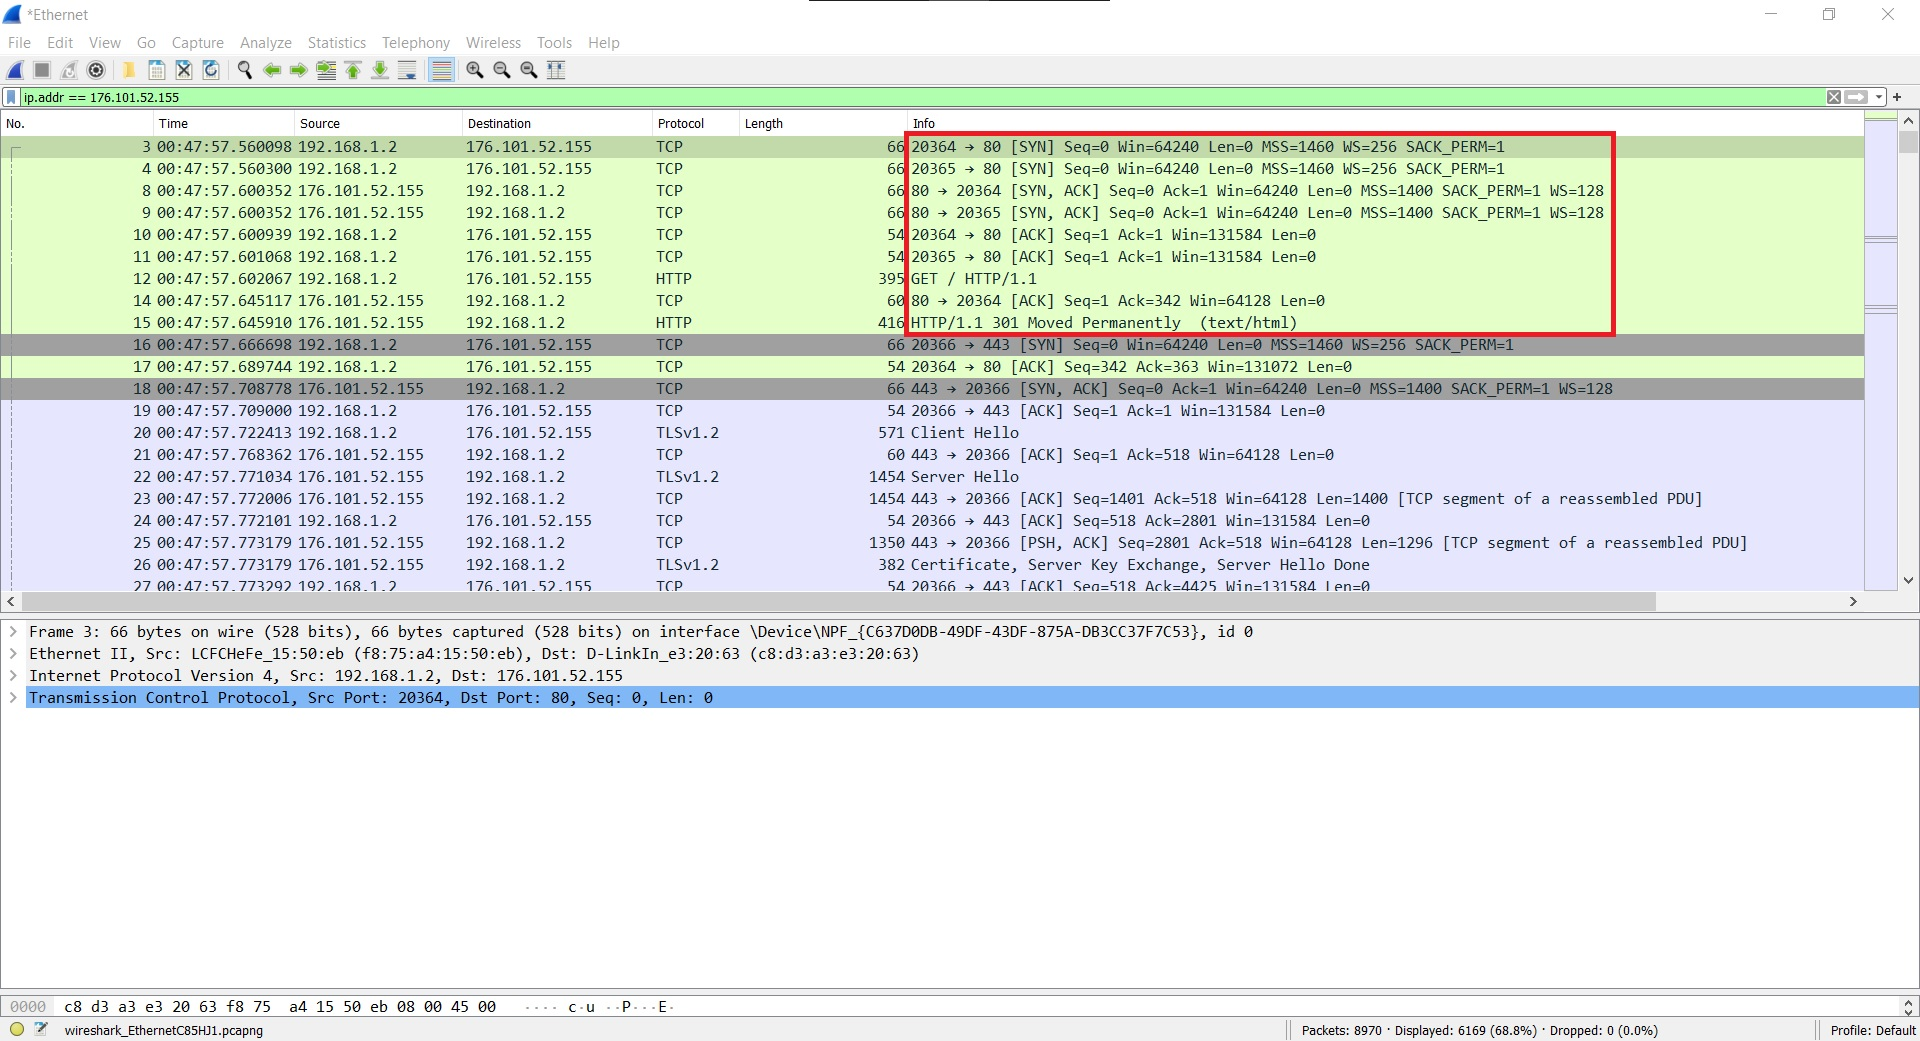
\includegraphics[width=1.0\textwidth]{figures/56.jpg}
    \caption{}
    \label{fig:fig1}
\end{figure}
پس از دریافت پاسخ از \lr{DNS query} مکانیسم \lr{TCP 3-Way Handshake} اتفاق می‌افتد و می‌بینیم که آدرس آی‌پی مقصدِ \lr{SYN} با آدرس آی‌پی ارائه شده در پیام \lr{DNS response} مطابقت دارد.
\subsection{}
بستگی به صفحه‌ی وب دارد. اگر صفحه دارای تصاویری از سایت‌های دیگر باشد به ازای هر سایت متمایز نیاز به یک \lr{DNS query} جدید می‌باشد.


\section{}
\subsection{}
\subsection{}
\subsection{}
\begin{figure}[H]
    \centering
    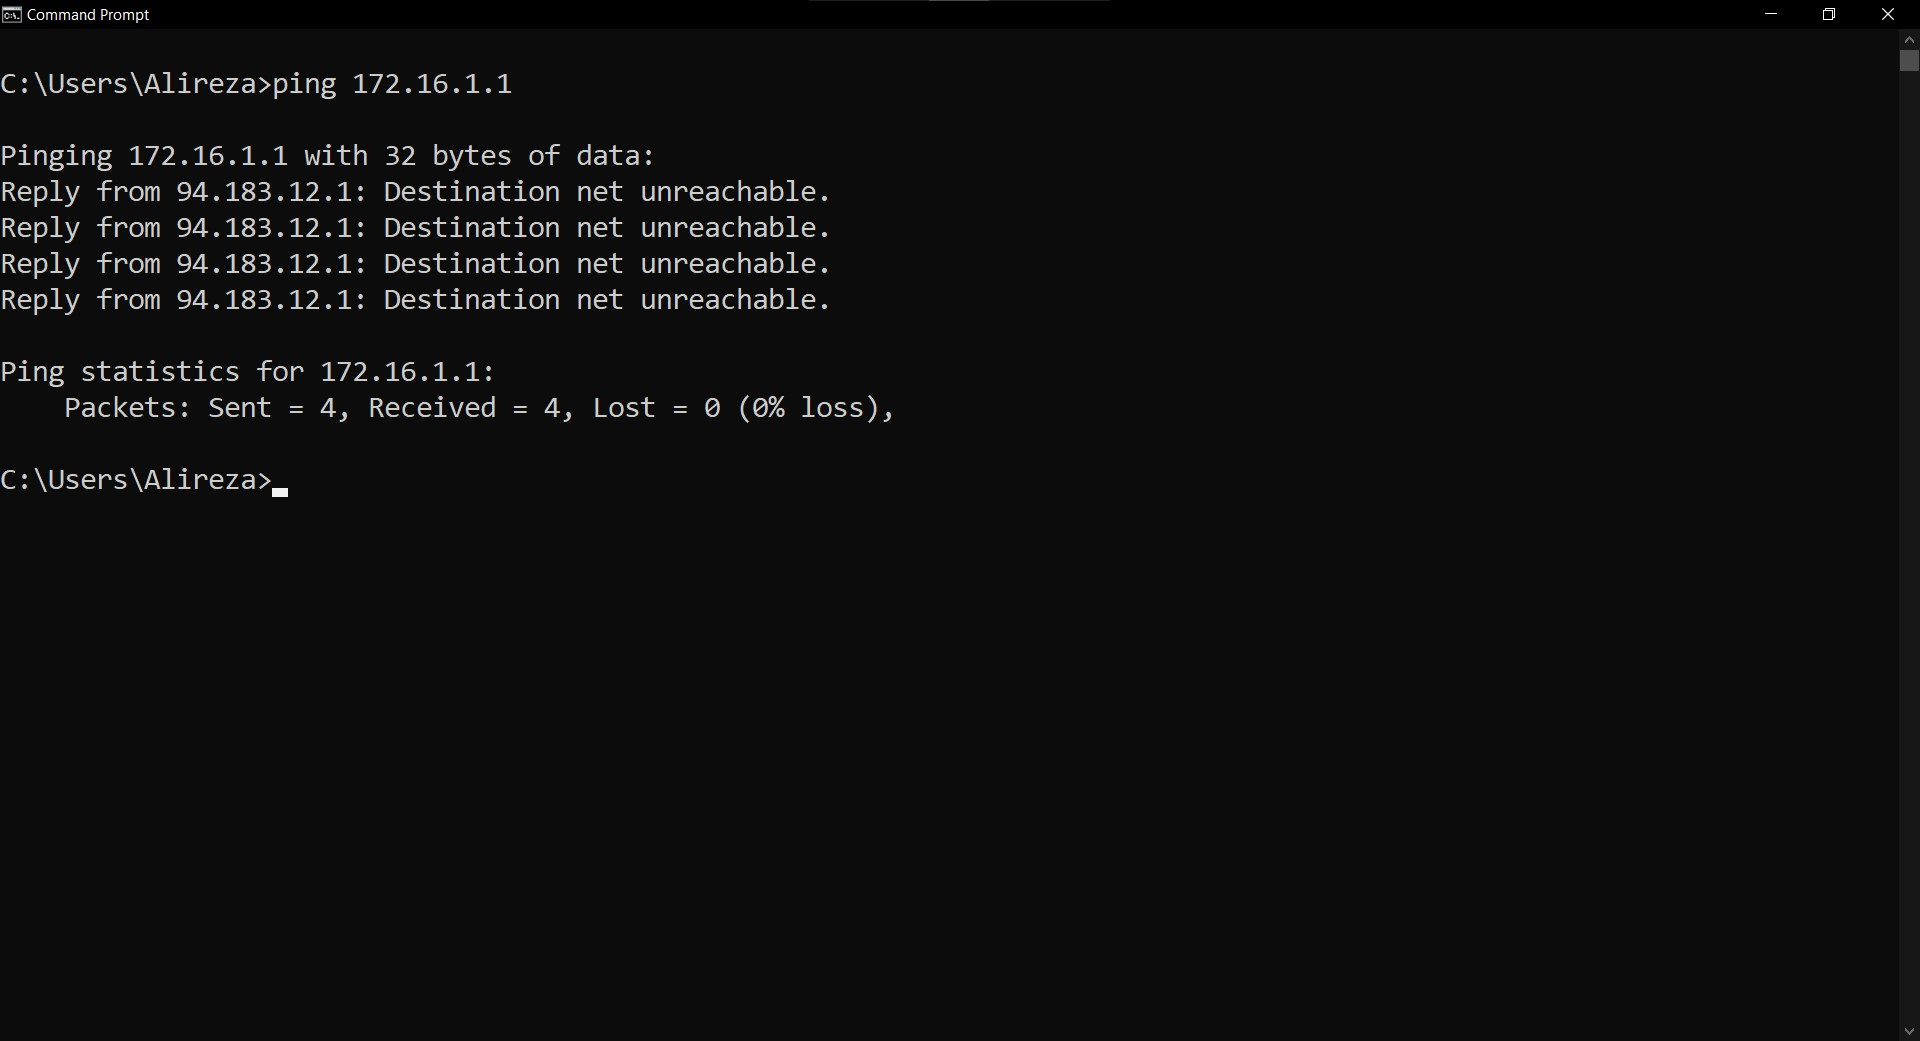
\includegraphics[width=1.0\textwidth]{figures/57.jpg}
    \caption{}
    \label{fig:fig1}
\end{figure}
\subsection{}
\begin{figure}[H]
    \centering
    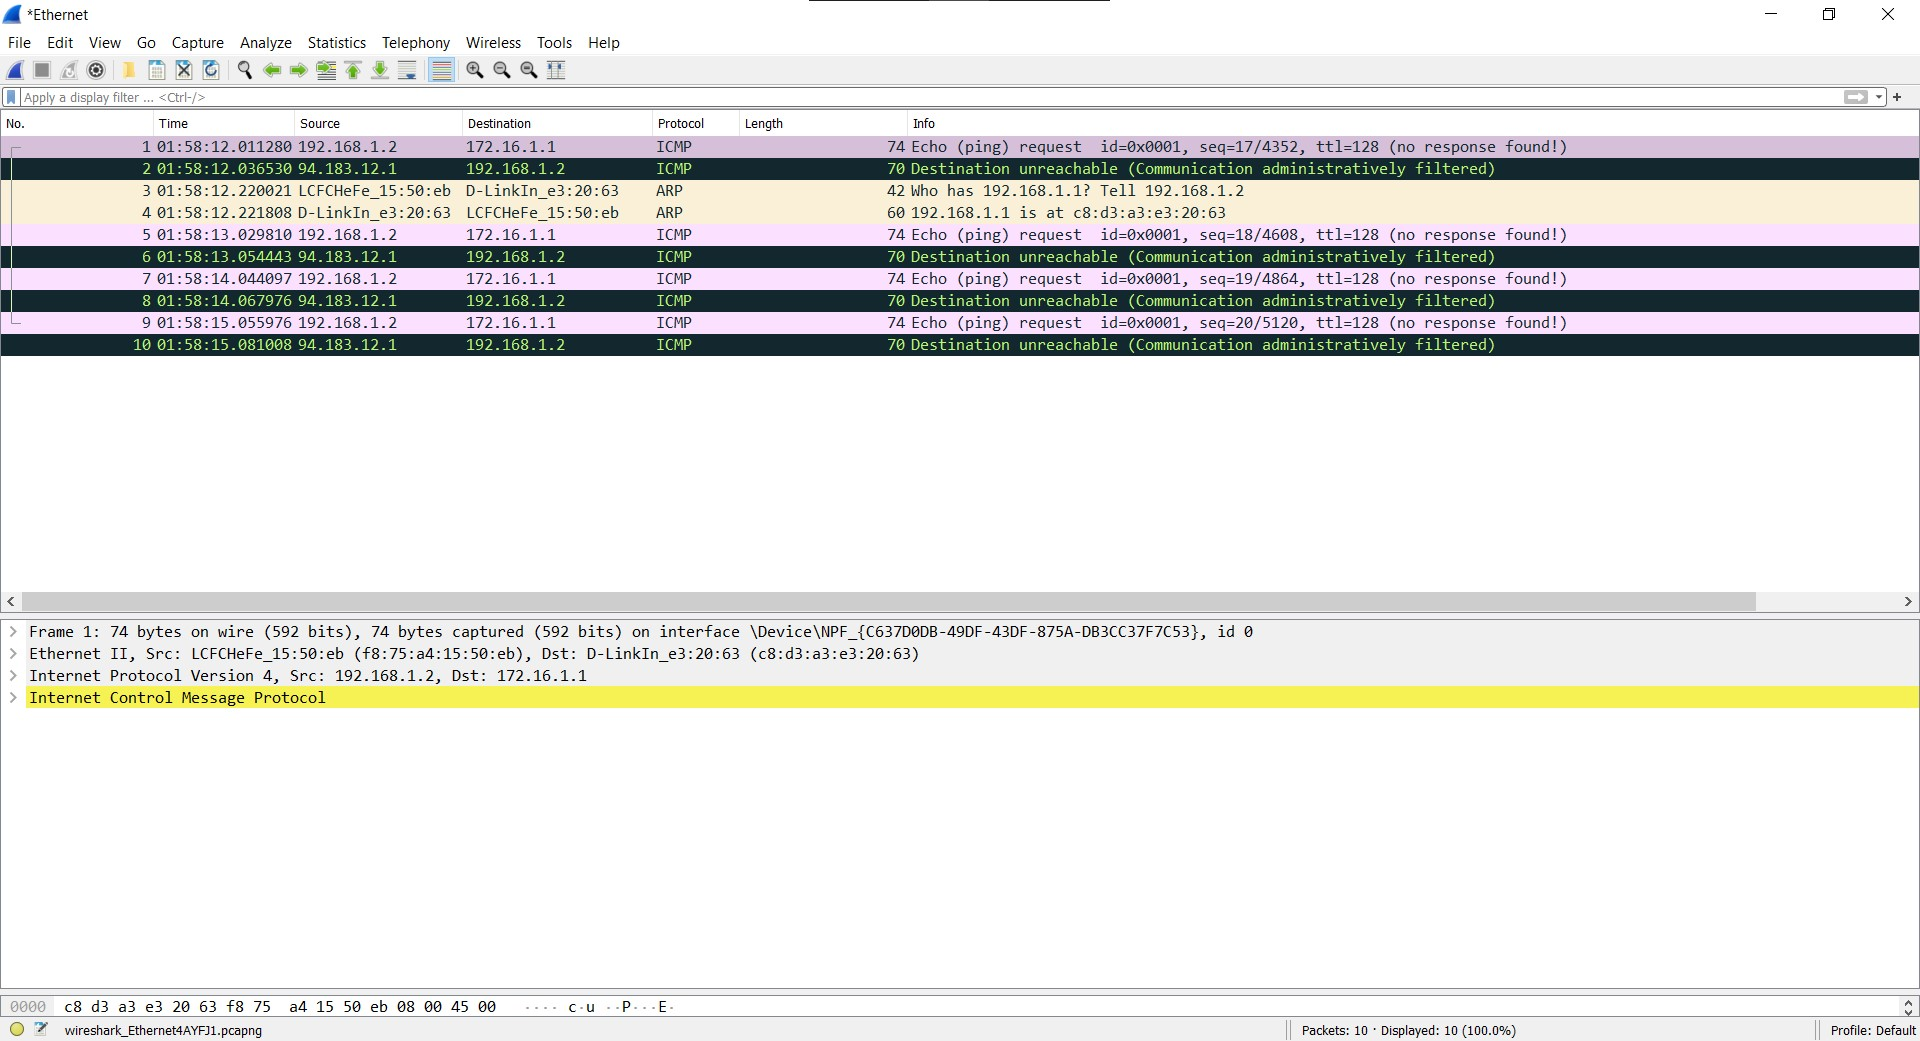
\includegraphics[width=1.0\textwidth]{figures/58.jpg}
    \caption{}
    \label{fig:fig1}
\end{figure}
دستور پینگ از پروتکل \lr{ICMP} استفاده می‌کند.

\subsection{}
فایل پیوست مشاهده شود.
\subsection{}
نحوه‌ی ذخیره کردن بسته‌های دلخواه:
\begin{figure}[H]
    \centering
    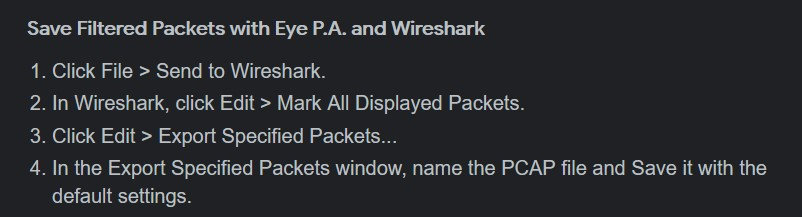
\includegraphics[width=1.0\textwidth]{figures/59.jpg}
    \caption{}
    \label{fig:fig1}
\end{figure}
فایل پیوست مشاهده ‌شود.
%%%%%%%%%%%%%%%%%%%%%%%%%%%%%%%%%%%%%%%%%%%%%%

\section*{منابع}
\renewcommand{\section}[2]{}%
\begin{thebibliography}{99} % assumes less than 100 references
%چنانچه مرجع فارسی نیز داشته باشید باید دستور فوق را فعال کنید و مراجع فارسی خود را بعد از این دستور وارد کنید


\begin{LTRitems}

\resetlatinfont

\bibitem{b1} https://stackoverflow.com/questions/246859/http-1-0-vs-1-1
\end{LTRitems}

\end{thebibliography}


\end{document}
